\documentclass{beamer}[10]
\usepackage{pgf}
\usepackage{beamerthemesplit}
\usepackage{array}
\usepackage{wrapfig}
\usepackage{varwidth}
%\usepackage{enumitem}
\usepackage{listings}
\lstset{language=bash,
	basicstyle=\ttfamily\scriptsize,		
	keywordstyle=\color{blue}\ttfamily,
	morekeywords={peter@kbpet},
	alsoletter={:~$},
	morekeywords=[2]{peter@kbpet:},
	keywordstyle=[2]{\color{red}},
	literate={\$}{{\textcolor{red}{\$}}}1 
	{:}{{\textcolor{red}{:}}}1
	{~}{{\textcolor{red}{\textasciitilde}}}1,
	breaklines=true,
	numbers=none,
	numbersep=5pt,
	stepnumber=1
}
\usepackage{algorithm,algpseudocode}
\usepackage{hyperref}
\usepackage{pdfpc-commands}
\usepackage{pgfpages}

\usepackage{tikz}
\usetikzlibrary{er,positioning}
\usepackage{float}
\usepackage{subcaption}
\usepackage{xcolor}
\usepackage[acronym,sort=def]{glossaries}

%\usepackage{natbib}
\bibliographystyle{apalike}

\definecolor{kugreen}{RGB}{50,93,61}
\definecolor{kugreenlys}{RGB}{132,158,139}
\definecolor{kugreenlyslys}{RGB}{173,190,177}
\definecolor{kugreenlyslyslys}{RGB}{214,223,216}
\definecolor{kublue}{RGB}{0,101,163}
\definecolor{kubluelys}{RGB}{132,158,139}
\definecolor{kubluelyslys}{RGB}{173,190,177}
\definecolor{kubluelyslyslys}{RGB}{214,223,216}
\setbeamercovered{transparent}
\mode<presentation>
\usetheme[numbers,totalnumber,compress,sidebarshades]{PaloAlto}
%\setbeamertemplate{footline}[frame number]

\usecolortheme[named=kublue]{structure}
\useinnertheme{circles}
\usefonttheme[onlymath]{serif}
\setbeamertemplate{blocks}[rounded][shadow=true]

% Define footer
\setbeamertemplate{footline}{bg=primary}
\makeatother
\setbeamertemplate{footline}
{
	\leavevmode%
	\hbox{%
		\begin{beamercolorbox}[wd=.4\paperwidth,ht=2.25ex,dp=1ex,right]{author in head/foot}%
		\usebeamerfont{author in head/foot}\insertshortauthor\ \quad \quad
		\end{beamercolorbox}%
		\begin{beamercolorbox}[wd=.6\paperwidth,ht=2.25ex,dp=1ex,left]{title in head/foot}%
		\usebeamerfont{title in head/foot}\quad \quad \insertshorttitle
		\hfill \hfill \hfill \hfill
		\insertframenumber{}/\inserttotalframenumber
		\end{beamercolorbox}}%
}
\makeatletter

\logo{
\includegraphics[width=1.5cm]{gfx/eth_logo_kurz_pos}}
\title{Map Fusion for Collaborative UAV SLAM}
\subtitle{Map Fusion for Collaborative UAV SLAM}
\author{Andreas Ziegler}
\institute{V4RL \\ ETH Zürich}
\date{12th of January 2017}

\newcommand{\setlistspacing}[2]{\def\@ld{#1}\expandafter\def\csname
	@list\romannumeral\@ld \endcsname{\leftmargin\csname
		leftmargin\romannumeral\@ld \endcsname
		\topsep    #2
		\parsep    0\p@   \@plus\p@
		\itemsep   #2}}
\makeatother

\newacronym{slam}{SLAM}{Simultaneous Localisation and Mapping}
\newacronym{uav}{UAV}{Unmanned Aerial Vehicle}

\newacronym{kf}{KF}{KeyFrame}
\newacronym[longplural={KeyFrame Matches}]{kfm}{KFM}{KeyFrame Match}

\newacronym{ba}{BA}{Bundle Adjustment}
\newacronym{pgo}{PGO}{Pose Graph Optimization}

\newacronym{lm}{LM}{Levenberg-Marquardt}
\newacronym{dl}{DL}{Powell's dog leg}

\makeglossaries
\setcounter{tocdepth}{1}

\begin{document}

\begin{frame}
	\frametitle{Semester Project}
	\begin{center}
	\LARGE Semester Project \\
	- \\
	Map Fusion for Collaborative UAV SLAM\\
	- \\
	\includegraphics*[height=0.6cm]{gfx/eth_logo_kurz_pos.eps} \hfill
	\includegraphics*[height=0.6cm]{gfx/v4rl_logo} \hfill
	\includegraphics*[height=0.6cm]{gfx/asl_logo_right.pdf}
	\end{center}
\end{frame}

\begin{frame}
	\frametitle{Contents}
	\tableofcontents
\end{frame}

\frame{ \frametitle{Acronyms}
  %\printglossaries
  \printglossary[nonumberlist,type=\acronymtype]
}

\section{Introduction}
\frame{\tableofcontents[currentsection]}

\frame{ \frametitle{Introduction}
	\only<1>{
  \begin{figure}[H]
    \centering
    \includegraphics*[scale=0.8]{gfx/uav_collaborative}
  \end{figure}
  }

  \only<2>{
  \begin{figure}[H]
    \centering
    \includegraphics*[scale=0.4]{gfx/map_1_2_1}
  \end{figure}
  }
  \only<3>{
  \begin{figure}[H]
    \centering
    \includegraphics*[scale=0.4]{gfx/map_1_2_2}
  \end{figure}
  }
  \only<4>{
  \begin{figure}[H]
    \centering
    \includegraphics*[scale=0.3]{gfx/map_1_2_merge}
  \end{figure}
  }
}
\note[enumerate]
{
  \item \acrshort{slam} is one of the most important challenges for robots to be autonomous
  \item For a team of \glspl{uav} collaboratively performing tasks, a common map is required
  \item To build a common map from the maps of the \glspl{uav}, the maps need to be merged
	\item To merge two maps, the alignment of them has to be found
}

\begin{frame}
  \frametitle{Introduction - What is a \acrfull{kfm}?}
  \only<1->{
    \acrfullpl{kf}: The most ``representative'' poses\\ 
    \medskip
  }
  \only<2>{
  Two clients each with an own landmarks and \acrfullpl{kf}
  \begin{center}
  \begin{tikzpicture}
    \coordinate (A) at (0, 0);
    \coordinate (B) at (3, 2);
    \coordinate (C) at (5, 2);
    \coordinate (D1) at (1, 1);
    \coordinate (D2) at (6, 1);
    \coordinate (E) at (8, 0);

    \coordinate (F) at (0.9, 0.9);
    \coordinate (G) at (0.8, 1.1);
    \coordinate (H) at (1.1, 1.1);

    \node at (A) {};
    \node at (B) {};
    \node at (C) {};
    \node at (E) {};

    \draw [orange!70, line width=0.5cm] (A) to [out=80, in=150] (D1);
    \draw [orange!70, line width=0.5cm] (D1) to [out=-20, in=-70] (B);
    \draw [blue!70, line width=0.5cm] (C) to [out=10, in=100] (D2);
    \draw [blue!70, line width=0.5cm] (D2) to [out=-80, in=70] (E);
    \draw [black] (A) to [out=80, in=150] (D1);
    \draw [black] (D1) to [out=-20, in=-70] (B);
    \draw [black] (C) to [out=10, in=100] (D2);
    \draw [black] (D2) to [out=-80, in=70] (E);

    \node [fill=black, circle,inner sep=1pt, text width=0.5mm] at (D1) {};
    \node [fill=black, circle,inner sep=1pt, text width=0.5mm] at (D2) {};
  \end{tikzpicture}
  \end{center}
  }
  \only<3>{
    \acrfull{kfm}: A pair of two \acrfullpl{kf} observing the same location\\
  }
  \only<4>{
    \acrfull{kfm}: Two \acrfullpl{kf} observing the same location $\rightarrow$ Can obtain transformation
  }
    
  \only<3-4>{
  \begin{center}
  \begin{tikzpicture}
    \coordinate (A) at (0, 0);
    \coordinate (B) at (3, 2);
    \coordinate (C) at (5, 2);
    \coordinate (D1) at (1, 1);
    \coordinate (D2) at (6, 1);
    \coordinate (E) at (8, 0);

    \coordinate (F) at (0.9, 0.9);
    \coordinate (G) at (0.8, 1.1);
    \coordinate (H) at (1.1, 1.1);

    \node at (A) {};
    \node at (B) {};
    \node at (C) {};
    \node at (E) {};

    \draw [orange!70, line width=0.5cm] (A) to [out=80, in=150] (D1);
    \draw [orange!70, line width=0.5cm] (D1) to [out=-20, in=-70] (B);
    \draw [blue!70, line width=0.5cm] (C) to [out=10, in=100] (D2);
    \draw [blue!70, line width=0.5cm] (D2) to [out=-80, in=70] (E);
    \draw [black] (A) to [out=80, in=150] (D1);
    \draw [black] (D1) to [out=-20, in=-70] (B);
    \draw [black] (C) to [out=10, in=100] (D2);
    \draw [black] (D2) to [out=-80, in=70] (E);

    \node [fill=black, circle,inner sep=1pt, text width=0.5mm] at (D1) {};
    \node [fill=black, circle,inner sep=1pt, text width=0.5mm] at (D2) {};

    \draw [red!50, line width=0.05cm, dashed] (D1) to (D2);
  \end{tikzpicture}
  \end{center}
  }
  \only<5>{
  \acrfull{kfm}: Two \acrfullpl{kf} observing the same location\\
  \medskip
  With the transformation $\rightarrow$ maps can be aligned
  \begin{center}
  \begin{tikzpicture}
    \coordinate (A) at (0, 0);
    \coordinate (B) at (3, 2);
    \coordinate (C) at (0, 2);
    \coordinate (D) at (1, 1);
    \coordinate (E) at (3, 0);

    \coordinate (F) at (0.9, 0.9);
    \coordinate (G) at (0.8, 1.1);
    \coordinate (H) at (1.1, 1.1);

    \node at (A) {};
    \node at (B) {};
    \node at (C) {};
    \node at (E) {};

    \draw [orange!70, line width=0.5cm] (A) to [out=80, in=150] (D);
    \draw [orange!70, line width=0.5cm] (D) to [out=-20, in=-70] (B);
    \draw [blue!70, line width=0.5cm] (C) to [out=10, in=100] (D);
    \draw [blue!70, line width=0.5cm] (D) to [out=-80, in=70] (E);
    \draw [black] (A) to [out=80, in=150] (D);
    \draw [black] (D) to [out=-20, in=-70] (B);
    \draw [black] (C) to [out=10, in=100] (D);
    \draw [black] (D) to [out=-80, in=70] (E);

    \node [fill=black, circle,inner sep=1pt, text width=0.5mm] at (D) {};
  \end{tikzpicture}
  \end{center}
  }
  \only<6>{
  A \acrfull{kfm} contains:
  \begin{itemize}
    \item Two \acrfullpl{kf} (One per map)
    \item The transformation ($T \in \text{Sim(3)}$) between them
  \end{itemize}

  \begin{center}
  \begin{tikzpicture}
    \coordinate (A) at (0, 0);
    \coordinate (B) at (3, 2);
    \coordinate (C) at (0, 2);
    \coordinate (D) at (1, 1);
    \coordinate (E) at (3, 0);

    \coordinate (F) at (0.9, 0.9);
    \coordinate (G) at (0.8, 1.1);
    \coordinate (H) at (1.1, 1.1);

    \node at (A) {};
    \node at (B) {};
    \node at (C) {};
    \node at (E) {};

    \draw [orange!70, line width=0.5cm] (A) to [out=80, in=150] (D);
    \draw [orange!70, line width=0.5cm] (D) to [out=-20, in=-70] (B);
    \draw [blue!70, line width=0.5cm] (C) to [out=10, in=100] (D);
    \draw [blue!70, line width=0.5cm] (D) to [out=-80, in=70] (E);
    \draw [black] (A) to [out=80, in=150] (D);
    \draw [black] (D) to [out=-20, in=-70] (B);
    \draw [black] (C) to [out=10, in=100] (D);
    \draw [black] (D) to [out=-80, in=70] (E);

    \node [fill=black, circle,inner sep=1pt, text width=0.5mm] at (D) {};
  \end{tikzpicture}
  \end{center}
  }
\end{frame}

\section{Motivation}
\frame{\tableofcontents[currentsection]}

\frame{ \frametitle{Motivation}
	\begin{itemize}
  \visible<1->{
  \item A multi agent SLAM system based on ORB-SLAM2 should be extended
  }
  \visible<2->{
  \item So far, as soon as a \acrfull{kfm} was detected, maps were merged
  }
  \visible<3->{
  \item Using multiple \glspl{kfm} to guarantee no false map merging
  }
  \visible<4->{
  \item Using multiple \glspl{kfm} to obtain an optimal map alignment
  }
  \end{itemize}
  \visible<1->{\tiny{\cite{Mur-Artal2016}}}
}

\section{Map merging}
\frame{\tableofcontents[currentsection]}

\subsection{Approaches}
\frame{	\frametitle{Map merging - Old approach}
   Old approach:
	\begin{itemize}
    \item As soon as a \gls{kfm} was detected, maps were merged
	\end{itemize}
}

\frame{
  \frametitle{Map merging - New approach}
  \only<1>{
  Find $n (= 3)$ \acrfullpl{kfm}
  \begin{center}
  \begin{tikzpicture}
    \coordinate (A1) at (0, 3);
    \coordinate (A1MP1) at (-0.5, 3.5);
    \coordinate (A1MP2) at (0, 3.75);
    \coordinate (A1MP3) at (0.5, 3.5);

    \coordinate (A2) at (0, 0);
    \coordinate (A2MP1) at (-0.5, 0.5);
    \coordinate (A2MP2) at (0, 0.75);
    \coordinate (A2MP3) at (0.5, 0.5);

    \node [fill=green!70, circle,inner sep=2pt, text width=0.1mm] at (A1MP1) {};
    \node [fill=green!70, circle,inner sep=2pt, text width=0.1mm] at (A1MP2) {};
    \node [fill=green!70, circle,inner sep=2pt, text width=0.1mm] at (A1MP3) {};
    \draw [green!50, dashed, line width=0.05cm] (A1) to (A1MP1);
    \draw [green!50, dashed, line width=0.05cm] (A1) to (A1MP2);
    \draw [green!50, dashed, line width=0.05cm] (A1) to (A1MP3);
    \node [fill=orange!70, circle,inner sep=2pt, text width=0.1mm] at (A1) {};

    \node [fill=green!70, circle,inner sep=2pt, text width=0.1mm] at (A2MP1) {};
    \node [fill=green!70, circle,inner sep=2pt, text width=0.1mm] at (A2MP2) {};
    \node [fill=green!70, circle,inner sep=2pt, text width=0.1mm] at (A2MP3) {};
    \draw [green!50, dashed, line width=0.05cm] (A2) to (A2MP1);
    \draw [green!50, dashed, line width=0.05cm] (A2) to (A2MP2);
    \draw [green!50, dashed, line width=0.05cm] (A2) to (A2MP3);
    \node [fill=blue!70, circle,inner sep=2pt, text width=0.1mm] at (A2) {};

    \node[draw] at (0.5, 5.3)
    {
    \scriptsize
    \begin{tabular}{cl}
      \tikz\node[fill=orange!70, circle,inner sep=3pt, text width=0.1mm] {}; \tikz\node[fill=blue!70, circle,inner sep=3pt, text width=0.1mm] {}; & KeyFrames of a Match \\
      \tikz\node[fill=orange!30, circle,inner sep=2pt, text width=0.1mm] {}; \tikz\node[fill=blue!30, circle,inner sep=2pt, text width=0.1mm] {}; & Skipped KeyFrames \\
      \tikz\node [fill=green!70, circle, inner sep=2pt, text width=0.1mm] {}; \tikz\node[fill=green!30, circle,inner sep=1pt, text width=0.1mm] {}; & Map Points (Landmarks)
    \end{tabular}
    };

  \end{tikzpicture}
  \end{center}
  }
  \only<2>{
  Find $n (= 3)$ \acrfullpl{kfm},\\
  Skip $m (= 5)$ \acrfullpl{kf}
  \begin{center}
  \begin{tikzpicture}
    \coordinate (A1) at (0, 3);
    \coordinate (A1MP1) at (-0.5, 3.5);
    \coordinate (A1MP2) at (0, 3.75);
    \coordinate (A1MP3) at (0.5, 3.5);

    \coordinate (A2) at (0, 0);
    \coordinate (A2MP1) at (-0.5, 0.5);
    \coordinate (A2MP2) at (0, 0.75);
    \coordinate (A2MP3) at (0.5, 0.5);

    \node [fill=green!70, circle,inner sep=2pt, text width=0.1mm] at (A1MP1) {};
    \node [fill=green!70, circle,inner sep=2pt, text width=0.1mm] at (A1MP2) {};
    \node [fill=green!70, circle,inner sep=2pt, text width=0.1mm] at (A1MP3) {};
    \draw [green!50, dashed, line width=0.05cm] (A1) to (A1MP1);
    \draw [green!50, dashed, line width=0.05cm] (A1) to (A1MP2);
    \draw [green!50, dashed, line width=0.05cm] (A1) to (A1MP3);
    \node [fill=orange!70, circle,inner sep=3pt, text width=0.1mm] at (A1) {};

    \node [fill=green!70, circle,inner sep=2pt, text width=0.1mm] at (A2MP1) {};
    \node [fill=green!70, circle,inner sep=2pt, text width=0.1mm] at (A2MP2) {};
    \node [fill=green!70, circle,inner sep=2pt, text width=0.1mm] at (A2MP3) {};
    \draw [green!50, dashed, line width=0.05cm] (A2) to (A2MP1);
    \draw [green!50, dashed, line width=0.05cm] (A2) to (A2MP2);
    \draw [green!50, dashed, line width=0.05cm] (A2) to (A2MP3);
    \node [fill=blue!70, circle,inner sep=3pt, text width=0.1mm] at (A2) {};

    \draw [red!50, line width=0.05cm, dashed] (A1) to (A2);

    \node[draw] at (0.5, 5.3)
    {
    \scriptsize
    \begin{tabular}{cl}
      \tikz\node[fill=orange!70, circle,inner sep=3pt, text width=0.1mm] {}; \tikz\node[fill=blue!70, circle,inner sep=3pt, text width=0.1mm] {}; & KeyFrames of a Match \\
      \tikz\node[fill=orange!30, circle,inner sep=2pt, text width=0.1mm] {}; \tikz\node[fill=blue!30, circle,inner sep=2pt, text width=0.1mm] {}; & Skipped KeyFrames \\
      \tikz\node [fill=green!70, circle, inner sep=2pt, text width=0.1mm] {}; \tikz\node[fill=green!30, circle,inner sep=1pt, text width=0.1mm] {}; & Map Points (Landmarks)
    \end{tabular}
    };

  \end{tikzpicture}
  \end{center}
  }

  \only<3>{
  Find $n (= 3)$ \acrfullpl{kfm},\\
  Skip $m (= 5)$ \acrfullpl{kf}
  \begin{center}
  \begin{tikzpicture}
    \coordinate (A1) at (0, 3);
    \coordinate (A1MP1) at (-0.5, 3.5);
    \coordinate (A1MP2) at (0, 3.75);
    \coordinate (A1MP3) at (0.5, 3.5);

    \coordinate (AB11) at (4/3, 3);
    \coordinate (AB11MP1) at (-0.25+4/3, 3.25);
    \coordinate (AB11MP2) at (4/3, 3.5);
    \coordinate (AB11MP3) at (0.25+4/3, 3.25);

    \coordinate (AB12) at (8/3, 3);
    \coordinate (AB12MP1) at (-0.25+8/3, 3.25);
    \coordinate (AB12MP2) at (8/3, 3.5);
    \coordinate (AB12MP3) at (0.25+8/3, 3.25);

    \coordinate (B1) at (4, 3);
    \coordinate (B1MP1) at (3.2, 3.15);
    \coordinate (B1MP2) at (3.4, 3.6);
    \coordinate (B1MP3) at (3.9, 3.5);

    \coordinate (A2) at (0, 0);
    \coordinate (A2MP1) at (-0.5, 0.5);
    \coordinate (A2MP2) at (0, 0.75);
    \coordinate (A2MP3) at (0.5, 0.5);

    \coordinate (AB21) at (2, 0);
    \coordinate (AB21MP1) at (1.75, 0.25);
    \coordinate (AB21MP2) at (2, 0.5);
    \coordinate (AB21MP3) at (2.25, 0.25);

    \coordinate (AB22) at (4, 0);
    \coordinate (AB22MP1) at (3.75, 0.25);
    \coordinate (AB22MP2) at (4, 0.5);
    \coordinate (AB22MP3) at (4.25, 0.25);

    \coordinate (AB23) at (6, 0);
    \coordinate (AB23MP1) at (5.75, 0.25);
    \coordinate (AB23MP2) at (6, 0.5);
    \coordinate (AB23MP3) at (6.25, 0.25);

    \coordinate (B2) at (8, 0);
    \coordinate (B2MP1) at (7.2, 0.15);
    \coordinate (B2MP2) at (7.4, 0.6);
    \coordinate (B2MP3) at (7.9, 0.5);


    \node [fill=green!30, circle,inner sep=2pt, text width=0.1mm] at (A1MP1) {};
    \node [fill=green!30, circle,inner sep=2pt, text width=0.1mm] at (A1MP2) {};
    \node [fill=green!30, circle,inner sep=2pt, text width=0.1mm] at (A1MP3) {};
    \draw [green!50, line width=0.05cm] (A1) to (A1MP1);
    \draw [green!50, line width=0.05cm] (A1) to (A1MP2);
    \draw [green!50, line width=0.05cm] (A1) to (A1MP3);
    \node [fill=orange!70, circle,inner sep=3pt, text width=0.1mm] at (A1) {};

    \node [fill=orange!30, circle,inner sep=1.5pt, text width=0.1mm] at (AB11) {};
    \node [fill=green!30, circle,inner sep=1pt, text width=0.1mm] at (AB11MP1) {};
    \node [fill=green!30, circle,inner sep=1pt, text width=0.1mm] at (AB11MP2) {};
    \node [fill=green!30, circle,inner sep=1pt, text width=0.1mm] at (AB11MP3) {};
    \draw [green!50, dashed, line width=0.025cm] (AB11) to (AB11MP1);
    \draw [green!50, dashed, line width=0.025cm] (AB11) to (AB11MP2);
    \draw [green!50, dashed, line width=0.025cm] (AB11) to (AB11MP3);

    \node [fill=orange!30, circle,inner sep=1.5pt, text width=0.1mm] at (AB12) {};
    \node [fill=green!30, circle,inner sep=1pt, text width=0.1mm] at (AB12MP1) {};
    \node [fill=green!30, circle,inner sep=1pt, text width=0.1mm] at (AB12MP2) {};
    \node [fill=green!30, circle,inner sep=1pt, text width=0.1mm] at (AB12MP3) {};
    \draw [green!50, dashed, line width=0.025cm] (AB12) to (AB12MP1);
    \draw [green!50, dashed, line width=0.025cm] (AB12) to (AB12MP2);
    \draw [green!50, dashed, line width=0.025cm] (AB12) to (AB12MP3);

    \node [fill=orange!70, circle,inner sep=2pt, text width=0.1mm] at (B1) {};
    \node [fill=green!30, circle, inner sep=2pt, text width=0.1mm] at (B1MP1) {};
    \node [fill=green!30, circle, inner sep=2pt, text width=0.1mm] at (B1MP2) {};
    \node [fill=green!30, circle, inner sep=2pt, text width=0.1mm] at (B1MP3) {};
    \draw [green!50, line width=0.05cm] (B1) to (B1MP1);
    \draw [green!50, line width=0.05cm] (B1) to (B1MP2);
    \draw [green!50, line width=0.05cm] (B1) to (B1MP3);

    \node [fill=blue!70, circle,inner sep=3pt, text width=0.1mm] at (A2) {};
    \node [fill=green!70, circle,inner sep=2pt, text width=0.1mm] at (A2MP1) {};
    \node [fill=green!70, circle,inner sep=2pt, text width=0.1mm] at (A2MP2) {};
    \node [fill=green!70, circle,inner sep=2pt, text width=0.1mm] at (A2MP3) {};
    \draw [green!50, dashed, line width=0.05cm] (A2) to (A2MP1);
    \draw [green!50, dashed, line width=0.05cm] (A2) to (A2MP2);
    \draw [green!50, dashed, line width=0.05cm] (A2) to (A2MP3);

    \node [fill=blue!30, circle,inner sep=2pt, text width=0.1mm] at (AB21) {};
    \node [fill=green!30, circle,inner sep=1pt, text width=0.1mm] at (AB21MP1) {};
    \node [fill=green!30, circle,inner sep=1pt, text width=0.1mm] at (AB21MP2) {};
    \node [fill=green!30, circle,inner sep=1pt, text width=0.1mm] at (AB21MP3) {};
    \draw [green!50, dashed, line width=0.025cm] (AB21) to (AB21MP1);
    \draw [green!50, dashed, line width=0.025cm] (AB21) to (AB21MP2);
    \draw [green!50, dashed, line width=0.025cm] (AB21) to (AB21MP3);

    \node [fill=blue!30, circle,inner sep=2pt, text width=0.1mm] at (AB22) {};
    \node [fill=green!30, circle,inner sep=1pt, text width=0.1mm] at (AB22MP1) {};
    \node [fill=green!30, circle,inner sep=1pt, text width=0.1mm] at (AB22MP2) {};
    \node [fill=green!30, circle,inner sep=1pt, text width=0.1mm] at (AB22MP3) {};
    \draw [green!50, dashed, line width=0.025cm] (AB22) to (AB22MP1);
    \draw [green!50, dashed, line width=0.025cm] (AB22) to (AB22MP2);
    \draw [green!50, dashed, line width=0.025cm] (AB22) to (AB22MP3);

    \node [fill=blue!30, circle,inner sep=2pt, text width=0.1mm] at (AB23) {};
    \node [fill=green!30, circle,inner sep=1pt, text width=0.1mm] at (AB23MP1) {};
    \node [fill=green!30, circle,inner sep=1pt, text width=0.1mm] at (AB23MP2) {};
    \node [fill=green!30, circle,inner sep=1pt, text width=0.1mm] at (AB23MP3) {};
    \draw [green!50, dashed, line width=0.025cm] (AB23) to (AB23MP1);
    \draw [green!50, dashed, line width=0.025cm] (AB23) to (AB23MP2);
    \draw [green!50, dashed, line width=0.025cm] (AB23) to (AB23MP3);

    \node [fill=blue!70, circle,inner sep=2pt, text width=0.1mm] at (B2) {};
    \node [fill=green!70, circle,inner sep=2pt, text width=0.1mm] at (B2MP1) {};
    \node [fill=green!70, circle,inner sep=2pt, text width=0.1mm] at (B2MP2) {};
    \node [fill=green!70, circle,inner sep=2pt, text width=0.1mm] at (B2MP3) {};
    \draw [green!50, dashed, line width=0.05cm] (B2) to (B2MP1);
    \draw [green!50, dashed, line width=0.05cm] (B2) to (B2MP2);
    \draw [green!50, dashed, line width=0.05cm] (B2) to (B2MP3);

    \draw [orange!50, line width=0.05cm] (A1) to (B1);
    \draw [blue!50, line width=0.05cm] (A2) to (B2);

    \draw [red!50, line width=0.05cm, dashed] (A1) to (A2);

    \node[draw] at (0.25, 5.0)
    {
    \scriptsize
    \begin{tabular}{cl}
      \tikz\node[fill=orange!70, circle,inner sep=3pt, text width=0.1mm] {}; \tikz\node[fill=blue!70, circle,inner sep=3pt, text width=0.1mm] {}; & KeyFrames of a Match \\
      \tikz\node[fill=orange!30, circle,inner sep=2pt, text width=0.1mm] {}; \tikz\node[fill=blue!30, circle,inner sep=2pt, text width=0.1mm] {}; & Skipped KeyFrames \\
      \tikz\node [fill=green!70, circle, inner sep=2pt, text width=0.1mm] {}; \tikz\node[fill=green!30, circle,inner sep=1pt, text width=0.1mm] {}; & Map Points (Landmarks)
    \end{tabular}
    };
  \end{tikzpicture}
  \end{center}
  }

  \only<4>{
  Find $n (= 3)$ \acrfullpl{kfm},\\
  Skip $m (= 5)$ \acrfullpl{kf}
  \begin{center}
  \begin{tikzpicture}
    \coordinate (A1) at (0, 3);
    \coordinate (A1MP1) at (-0.5, 3.5);
    \coordinate (A1MP2) at (0, 3.75);
    \coordinate (A1MP3) at (0.5, 3.5);

    \coordinate (AB11) at (4/3, 3);
    \coordinate (AB11MP1) at (-0.25+4/3, 3.25);
    \coordinate (AB11MP2) at (4/3, 3.5);
    \coordinate (AB11MP3) at (0.25+4/3, 3.25);

    \coordinate (AB12) at (8/3, 3);
    \coordinate (AB12MP1) at (-0.25+8/3, 3.25);
    \coordinate (AB12MP2) at (8/3, 3.5);
    \coordinate (AB12MP3) at (0.25+8/3, 3.25);

    \coordinate (B1) at (4, 3);
    \coordinate (B1MP1) at (3.2, 3.15);
    \coordinate (B1MP2) at (3.4, 3.6);
    \coordinate (B1MP3) at (3.9, 3.5);

    \coordinate (A2) at (0, 0);
    \coordinate (A2MP1) at (-0.5, 0.5);
    \coordinate (A2MP2) at (0, 0.75);
    \coordinate (A2MP3) at (0.5, 0.5);

    \coordinate (AB21) at (2, 0);
    \coordinate (AB21MP1) at (1.75, 0.25);
    \coordinate (AB21MP2) at (2, 0.5);
    \coordinate (AB21MP3) at (2.25, 0.25);

    \coordinate (AB22) at (4, 0);
    \coordinate (AB22MP1) at (3.75, 0.25);
    \coordinate (AB22MP2) at (4, 0.5);
    \coordinate (AB22MP3) at (4.25, 0.25);

    \coordinate (AB23) at (6, 0);
    \coordinate (AB23MP1) at (5.75, 0.25);
    \coordinate (AB23MP2) at (6, 0.5);
    \coordinate (AB23MP3) at (6.25, 0.25);

    \coordinate (B2) at (8, 0);
    \coordinate (B2MP1) at (7.2, 0.15);
    \coordinate (B2MP2) at (7.4, 0.6);
    \coordinate (B2MP3) at (7.9, 0.5);


    \node [fill=green!30, circle,inner sep=2pt, text width=0.1mm] at (A1MP1) {};
    \node [fill=green!30, circle,inner sep=2pt, text width=0.1mm] at (A1MP2) {};
    \node [fill=green!30, circle,inner sep=2pt, text width=0.1mm] at (A1MP3) {};
    \draw [green!50, line width=0.05cm] (A1) to (A1MP1);
    \draw [green!50, line width=0.05cm] (A1) to (A1MP2);
    \draw [green!50, line width=0.05cm] (A1) to (A1MP3);
    \node [fill=orange!70, circle,inner sep=3pt, text width=0.1mm] at (A1) {};

    \node [fill=orange!30, circle,inner sep=1.5pt, text width=0.1mm] at (AB11) {};
    \node [fill=green!30, circle,inner sep=1pt, text width=0.1mm] at (AB11MP1) {};
    \node [fill=green!30, circle,inner sep=1pt, text width=0.1mm] at (AB11MP2) {};
    \node [fill=green!30, circle,inner sep=1pt, text width=0.1mm] at (AB11MP3) {};
    \draw [green!50, dashed, line width=0.025cm] (AB11) to (AB11MP1);
    \draw [green!50, dashed, line width=0.025cm] (AB11) to (AB11MP2);
    \draw [green!50, dashed, line width=0.025cm] (AB11) to (AB11MP3);

    \node [fill=orange!30, circle,inner sep=1.5pt, text width=0.1mm] at (AB12) {};
    \node [fill=green!30, circle,inner sep=1pt, text width=0.1mm] at (AB12MP1) {};
    \node [fill=green!30, circle,inner sep=1pt, text width=0.1mm] at (AB12MP2) {};
    \node [fill=green!30, circle,inner sep=1pt, text width=0.1mm] at (AB12MP3) {};
    \draw [green!50, dashed, line width=0.025cm] (AB12) to (AB12MP1);
    \draw [green!50, dashed, line width=0.025cm] (AB12) to (AB12MP2);
    \draw [green!50, dashed, line width=0.025cm] (AB12) to (AB12MP3);

    \node [fill=orange!70, circle,inner sep=3pt, text width=0.1mm] at (B1) {};
    \node [fill=green!30, circle, inner sep=2pt, text width=0.1mm] at (B1MP1) {};
    \node [fill=green!30, circle, inner sep=2pt, text width=0.1mm] at (B1MP2) {};
    \node [fill=green!30, circle, inner sep=2pt, text width=0.1mm] at (B1MP3) {};
    \draw [green!50, line width=0.05cm] (B1) to (B1MP1);
    \draw [green!50, line width=0.05cm] (B1) to (B1MP2);
    \draw [green!50, line width=0.05cm] (B1) to (B1MP3);

    \node [fill=blue!70, circle,inner sep=3pt, text width=0.1mm] at (A2) {};
    \node [fill=green!70, circle,inner sep=2pt, text width=0.1mm] at (A2MP1) {};
    \node [fill=green!70, circle,inner sep=2pt, text width=0.1mm] at (A2MP2) {};
    \node [fill=green!70, circle,inner sep=2pt, text width=0.1mm] at (A2MP3) {};
    \draw [green!50, dashed, line width=0.05cm] (A2) to (A2MP1);
    \draw [green!50, dashed, line width=0.05cm] (A2) to (A2MP2);
    \draw [green!50, dashed, line width=0.05cm] (A2) to (A2MP3);

    \node [fill=blue!30, circle,inner sep=2pt, text width=0.1mm] at (AB21) {};
    \node [fill=green!30, circle,inner sep=1pt, text width=0.1mm] at (AB21MP1) {};
    \node [fill=green!30, circle,inner sep=1pt, text width=0.1mm] at (AB21MP2) {};
    \node [fill=green!30, circle,inner sep=1pt, text width=0.1mm] at (AB21MP3) {};
    \draw [green!50, dashed, line width=0.025cm] (AB21) to (AB21MP1);
    \draw [green!50, dashed, line width=0.025cm] (AB21) to (AB21MP2);
    \draw [green!50, dashed, line width=0.025cm] (AB21) to (AB21MP3);

    \node [fill=blue!30, circle,inner sep=2pt, text width=0.1mm] at (AB22) {};
    \node [fill=green!30, circle,inner sep=1pt, text width=0.1mm] at (AB22MP1) {};
    \node [fill=green!30, circle,inner sep=1pt, text width=0.1mm] at (AB22MP2) {};
    \node [fill=green!30, circle,inner sep=1pt, text width=0.1mm] at (AB22MP3) {};
    \draw [green!50, dashed, line width=0.025cm] (AB22) to (AB22MP1);
    \draw [green!50, dashed, line width=0.025cm] (AB22) to (AB22MP2);
    \draw [green!50, dashed, line width=0.025cm] (AB22) to (AB22MP3);

    \node [fill=blue!30, circle,inner sep=2pt, text width=0.1mm] at (AB23) {};
    \node [fill=green!30, circle,inner sep=1pt, text width=0.1mm] at (AB23MP1) {};
    \node [fill=green!30, circle,inner sep=1pt, text width=0.1mm] at (AB23MP2) {};
    \node [fill=green!30, circle,inner sep=1pt, text width=0.1mm] at (AB23MP3) {};
    \draw [green!50, dashed, line width=0.025cm] (AB23) to (AB23MP1);
    \draw [green!50, dashed, line width=0.025cm] (AB23) to (AB23MP2);
    \draw [green!50, dashed, line width=0.025cm] (AB23) to (AB23MP3);

    \node [fill=blue!70, circle,inner sep=3pt, text width=0.1mm] at (B2) {};
    \node [fill=green!70, circle,inner sep=2pt, text width=0.1mm] at (B2MP1) {};
    \node [fill=green!70, circle,inner sep=2pt, text width=0.1mm] at (B2MP2) {};
    \node [fill=green!70, circle,inner sep=2pt, text width=0.1mm] at (B2MP3) {};
    \draw [green!50, dashed, line width=0.05cm] (B2) to (B2MP1);
    \draw [green!50, dashed, line width=0.05cm] (B2) to (B2MP2);
    \draw [green!50, dashed, line width=0.05cm] (B2) to (B2MP3);

    \draw [orange!50, line width=0.05cm] (A1) to (B1);
    \draw [blue!50, line width=0.05cm] (A2) to (B2);

    \draw [red!50, line width=0.05cm, dashed] (A1) to (A2);
    \draw [red!50, line width=0.05cm, dashed] (B1) to (B2);

    \node[draw] at (0.25, 5.0)
    {
    \scriptsize
    \begin{tabular}{cl}
      \tikz\node[fill=orange!70, circle,inner sep=3pt, text width=0.1mm] {}; \tikz\node[fill=blue!70, circle,inner sep=3pt, text width=0.1mm] {}; & KeyFrames of a Match \\
      \tikz\node[fill=orange!30, circle,inner sep=2pt, text width=0.1mm] {}; \tikz\node[fill=blue!30, circle,inner sep=2pt, text width=0.1mm] {}; & Skipped KeyFrames \\
      \tikz\node [fill=green!70, circle, inner sep=2pt, text width=0.1mm] {}; \tikz\node[fill=green!30, circle,inner sep=1pt, text width=0.1mm] {}; & Map Points (Landmarks)
    \end{tabular}
    };
  \end{tikzpicture}
  \end{center}
  }

  \only<5>{
  Find $n (= 3)$ \acrfullpl{kfm}, Skip $m (= 5)$ \acrshortpl{kf}
  
  \begin{center}
  \begin{tikzpicture}
    \coordinate (A1) at (0, 3);
    \coordinate (A1MP1) at (-0.5, 3.5);
    \coordinate (A1MP2) at (0, 3.75);
    \coordinate (A1MP3) at (0.5, 3.5);

    \coordinate (AB11) at (4/3, 3);
    \coordinate (AB11MP1) at (-0.25+4/3, 3.25);
    \coordinate (AB11MP2) at (4/3, 3.5);
    \coordinate (AB11MP3) at (0.25+4/3, 3.25);

    \coordinate (AB12) at (8/3, 3);
    \coordinate (AB12MP1) at (-0.25+8/3, 3.25);
    \coordinate (AB12MP2) at (8/3, 3.5);
    \coordinate (AB12MP3) at (0.25+8/3, 3.25);

    \coordinate (B1) at (4, 3);
    \coordinate (B1MP1) at (3.2, 3.15);
    \coordinate (B1MP2) at (3.4, 3.6);
    \coordinate (B1MP3) at (3.9, 3.5);

    \coordinate (BC11) at (4, 4);
    \coordinate (BC11MP1) at (3.75, 4.25);
    \coordinate (BC11MP2) at (3.5, 4.0);
    \coordinate (BC11MP3) at (3.75, 3.75);

    \coordinate (BC12) at (4, 5);
    \coordinate (BC12MP1) at (3.75, 5.25);
    \coordinate (BC12MP2) at (3.5, 5.0);
    \coordinate (BC12MP3) at (3.75, 4.75);

    \coordinate (C1) at (4, 6);
    \coordinate (C1MP1) at (3.5, 6.5);
    \coordinate (C1MP2) at (3.25, 6.0);
    \coordinate (C1MP3) at (3.5, 5.5);

    \coordinate (A2) at (0, 0);
    \coordinate (A2MP1) at (-0.5, 0.5);
    \coordinate (A2MP2) at (0, 0.75);
    \coordinate (A2MP3) at (0.5, 0.5);

    \coordinate (AB21) at (2, 0);
    \coordinate (AB21MP1) at (1.75, 0.25);
    \coordinate (AB21MP2) at (2, 0.5);
    \coordinate (AB21MP3) at (2.25, 0.25);

    \coordinate (AB22) at (4, 0);
    \coordinate (AB22MP1) at (3.75, 0.25);
    \coordinate (AB22MP2) at (4, 0.5);
    \coordinate (AB22MP3) at (4.25, 0.25);

    \coordinate (AB23) at (6, 0);
    \coordinate (AB23MP1) at (5.75, 0.25);
    \coordinate (AB23MP2) at (6, 0.5);
    \coordinate (AB23MP3) at (6.25, 0.25);

    \coordinate (B2) at (8, 0);
    \coordinate (B2MP1) at (7.2, 0.15);
    \coordinate (B2MP2) at (7.4, 0.6);
    \coordinate (B2MP3) at (7.9, 0.5);

    \coordinate (BC21) at (8, 1.5);
    \coordinate (BC21MP1) at (7.75, 1.75);
    \coordinate (BC21MP2) at (7.5, 1.5);
    \coordinate (BC21MP3) at (7.75, 1.25);

    \coordinate (BC22) at (8, 3);
    \coordinate (BC22MP1) at (7.75, 3.25);
    \coordinate (BC22MP2) at (7.5, 3.0);
    \coordinate (BC22MP3) at (7.75, 2.75);

    \coordinate (BC23) at (8, 4.5);
    \coordinate (BC23MP1) at (7.75, 4.75);
    \coordinate (BC23MP2) at (7.5, 4.5);
    \coordinate (BC23MP3) at (7.75, 4.25);

    \coordinate (C2) at (8, 6);
    \coordinate (C2MP1) at (7.5, 6.5);
    \coordinate (C2MP2) at (7.25, 6.0);
    \coordinate (C2MP3) at (7.5, 5.5);

    \node [fill=orange!70, circle,inner sep=3pt, text width=0.1mm] at (A1) {};
    \node [fill=green!70, circle,inner sep=2pt, text width=0.1mm] at (A1MP1) {};
    \node [fill=green!70, circle,inner sep=2pt, text width=0.1mm] at (A1MP2) {};
    \node [fill=green!70, circle,inner sep=2pt, text width=0.1mm] at (A1MP3) {};
    \draw [green!50, dashed, line width=0.05cm] (A1) to (A1MP1);
    \draw [green!50, dashed, line width=0.05cm] (A1) to (A1MP2);
    \draw [green!50, dashed, line width=0.05cm] (A1) to (A1MP3);

    \node [fill=orange!30, circle,inner sep=2pt, text width=0.1mm] at (AB11) {};
    \node [fill=green!30, circle,inner sep=1pt, text width=0.1mm] at (AB11MP1) {};
    \node [fill=green!30, circle,inner sep=1pt, text width=0.1mm] at (AB11MP2) {};
    \node [fill=green!30, circle,inner sep=1pt, text width=0.1mm] at (AB11MP3) {};
    \draw [green!50, dashed, line width=0.025cm] (AB11) to (AB11MP1);
    \draw [green!50, dashed, line width=0.025cm] (AB11) to (AB11MP2);
    \draw [green!50, dashed, line width=0.025cm] (AB11) to (AB11MP3);

    \node [fill=orange!30, circle,inner sep=2pt, text width=0.1mm] at (AB12) {};
    \node [fill=green!30, circle,inner sep=1pt, text width=0.1mm] at (AB12MP1) {};
    \node [fill=green!30, circle,inner sep=1pt, text width=0.1mm] at (AB12MP2) {};
    \node [fill=green!30, circle,inner sep=1pt, text width=0.1mm] at (AB12MP3) {};
    \draw [green!50, dashed, line width=0.025cm] (AB12) to (AB12MP1);
    \draw [green!50, dashed, line width=0.025cm] (AB12) to (AB12MP2);
    \draw [green!50, dashed, line width=0.025cm] (AB12) to (AB12MP3);

    \node [fill=orange!70, circle, inner sep=3pt, text width=0.1mm] at (B1) {};
    \node [fill=green!70, circle, inner sep=2pt, text width=0.1mm] at (B1MP1) {};
    \node [fill=green!70, circle, inner sep=2pt, text width=0.1mm] at (B1MP2) {};
    \node [fill=green!70, circle, inner sep=2pt, text width=0.1mm] at (B1MP3) {};
    \draw [green!50, dashed, line width=0.05cm] (B1) to (B1MP1);
    \draw [green!50, dashed, line width=0.05cm] (B1) to (B1MP2);
    \draw [green!50, dashed, line width=0.05cm] (B1) to (B1MP3);

    \node [fill=orange!30, circle, inner sep=2pt, text width=0.1mm] at (BC11) {};
    \node [fill=green!30, circle,inner sep=1pt, text width=0.1mm] at (BC11MP1) {};
    \node [fill=green!30, circle,inner sep=1pt, text width=0.1mm] at (BC11MP2) {};
    \node [fill=green!30, circle,inner sep=1pt, text width=0.1mm] at (BC11MP3) {};
    \draw [green!50, dashed, line width=0.025cm] (BC11) to (BC11MP1);
    \draw [green!50, dashed, line width=0.025cm] (BC11) to (BC11MP2);
    \draw [green!50, dashed, line width=0.025cm] (BC11) to (BC11MP3);

    \node [fill=orange!30, circle, inner sep=2pt, text width=0.1mm] at (BC12) {};
    \node [fill=green!30, circle,inner sep=1pt, text width=0.1mm] at (BC12MP1) {};
    \node [fill=green!30, circle,inner sep=1pt, text width=0.1mm] at (BC12MP2) {};
    \node [fill=green!30, circle,inner sep=1pt, text width=0.1mm] at (BC12MP3) {};
    \draw [green!50, dashed, line width=0.025cm] (BC12) to (BC12MP1);
    \draw [green!50, dashed, line width=0.025cm] (BC12) to (BC12MP2);
    \draw [green!50, dashed, line width=0.025cm] (BC12) to (BC12MP3);

    \node [fill=orange!70, circle,inner sep=2pt, text width=0.1mm] at (C1) {};
    \node [fill=green!70, circle, inner sep=2pt, text width=0.1mm] at (C1MP1) {};
    \node [fill=green!70, circle, inner sep=2pt, text width=0.1mm] at (C1MP2) {};
    \node [fill=green!70, circle, inner sep=2pt, text width=0.1mm] at (C1MP3) {};
    \draw [green!50, dashed, line width=0.05cm] (C1) to (C1MP1);
    \draw [green!50, dashed, line width=0.05cm] (C1) to (C1MP2);
    \draw [green!50, dashed, line width=0.05cm] (C1) to (C1MP3);

    \node [fill=blue!70, circle,inner sep=3pt, text width=0.1mm] at (A2) {};
    \node [fill=green!70, circle,inner sep=2pt, text width=0.1mm] at (A2MP1) {};
    \node [fill=green!70, circle,inner sep=2pt, text width=0.1mm] at (A2MP2) {};
    \node [fill=green!70, circle,inner sep=2pt, text width=0.1mm] at (A2MP3) {};
    \draw [green!50, dashed, line width=0.05cm] (A2) to (A2MP1);
    \draw [green!50, dashed, line width=0.05cm] (A2) to (A2MP2);
    \draw [green!50, dashed, line width=0.05cm] (A2) to (A2MP3);

    \node [fill=blue!30, circle,inner sep=2pt, text width=0.1mm] at (AB21) {};
    \node [fill=green!30, circle,inner sep=1pt, text width=0.1mm] at (AB21MP1) {};
    \node [fill=green!30, circle,inner sep=1pt, text width=0.1mm] at (AB21MP2) {};
    \node [fill=green!30, circle,inner sep=1pt, text width=0.1mm] at (AB21MP3) {};
    \draw [green!50, dashed, line width=0.025cm] (AB21) to (AB21MP1);
    \draw [green!50, dashed, line width=0.025cm] (AB21) to (AB21MP2);
    \draw [green!50, dashed, line width=0.025cm] (AB21) to (AB21MP3);

    \node [fill=blue!30, circle,inner sep=2pt, text width=0.1mm] at (AB22) {};
    \node [fill=green!30, circle,inner sep=1pt, text width=0.1mm] at (AB22MP1) {};
    \node [fill=green!30, circle,inner sep=1pt, text width=0.1mm] at (AB22MP2) {};
    \node [fill=green!30, circle,inner sep=1pt, text width=0.1mm] at (AB22MP3) {};
    \draw [green!50, dashed, line width=0.025cm] (AB22) to (AB22MP1);
    \draw [green!50, dashed, line width=0.025cm] (AB22) to (AB22MP2);
    \draw [green!50, dashed, line width=0.025cm] (AB22) to (AB22MP3);

    \node [fill=blue!30, circle,inner sep=2pt, text width=0.1mm] at (AB23) {};
    \node [fill=green!30, circle,inner sep=1pt, text width=0.1mm] at (AB23MP1) {};
    \node [fill=green!30, circle,inner sep=1pt, text width=0.1mm] at (AB23MP2) {};
    \node [fill=green!30, circle,inner sep=1pt, text width=0.1mm] at (AB23MP3) {};
    \draw [green!50, dashed, line width=0.025cm] (AB23) to (AB23MP1);
    \draw [green!50, dashed, line width=0.025cm] (AB23) to (AB23MP2);
    \draw [green!50, dashed, line width=0.025cm] (AB23) to (AB23MP3);

    \node [fill=blue!70, circle,inner sep=3pt, text width=0.1mm] at (B2) {};
    \node [fill=green!70, circle,inner sep=2pt, text width=0.1mm] at (B2MP1) {};
    \node [fill=green!70, circle,inner sep=2pt, text width=0.1mm] at (B2MP2) {};
    \node [fill=green!70, circle,inner sep=2pt, text width=0.1mm] at (B2MP3) {};
    \draw [green!50, dashed, line width=0.05cm] (B2) to (B2MP1);
    \draw [green!50, dashed, line width=0.05cm] (B2) to (B2MP2);
    \draw [green!50, dashed, line width=0.05cm] (B2) to (B2MP3);

    \node [fill=blue!30, circle,inner sep=2pt, text width=0.1mm] at (BC21) {};
    \node [fill=green!30, circle,inner sep=1pt, text width=0.1mm] at (BC21MP1) {};
    \node [fill=green!30, circle,inner sep=1pt, text width=0.1mm] at (BC21MP2) {};
    \node [fill=green!30, circle,inner sep=1pt, text width=0.1mm] at (BC21MP3) {};
    \draw [green!50, dashed, line width=0.025cm] (BC21) to (BC21MP1);
    \draw [green!50, dashed, line width=0.025cm] (BC21) to (BC21MP2);
    \draw [green!50, dashed, line width=0.025cm] (BC21) to (BC21MP3);

    \node [fill=blue!30, circle,inner sep=2pt, text width=0.1mm] at (BC22) {};
    \node [fill=green!30, circle,inner sep=1pt, text width=0.1mm] at (BC22MP1) {};
    \node [fill=green!30, circle,inner sep=1pt, text width=0.1mm] at (BC22MP2) {};
    \node [fill=green!30, circle,inner sep=1pt, text width=0.1mm] at (BC22MP3) {};
    \draw [green!50, dashed, line width=0.025cm] (BC22) to (BC22MP1);
    \draw [green!50, dashed, line width=0.025cm] (BC22) to (BC22MP2);
    \draw [green!50, dashed, line width=0.025cm] (BC22) to (BC22MP3);
    
    \node [fill=blue!30, circle,inner sep=2pt, text width=0.1mm] at (BC23) {};
    \node [fill=green!30, circle,inner sep=1pt, text width=0.1mm] at (BC23MP1) {};
    \node [fill=green!30, circle,inner sep=1pt, text width=0.1mm] at (BC23MP2) {};
    \node [fill=green!30, circle,inner sep=1pt, text width=0.1mm] at (BC23MP3) {};
    \draw [green!50, dashed, line width=0.025cm] (BC23) to (BC23MP1);
    \draw [green!50, dashed, line width=0.025cm] (BC23) to (BC23MP2);
    \draw [green!50, dashed, line width=0.025cm] (BC23) to (BC23MP3);

    \node [fill=blue!70, circle,inner sep=2pt, text width=0.1mm] at (C2) {};
    \node [fill=green!70, circle, inner sep=2pt, text width=0.1mm] at (C2MP1) {};
    \node [fill=green!70, circle, inner sep=2pt, text width=0.1mm] at (C2MP2) {};
    \node [fill=green!70, circle, inner sep=2pt, text width=0.1mm] at (C2MP3) {};
    \draw [green!50, dashed, line width=0.05cm] (C2) to (C2MP1);
    \draw [green!50, dashed, line width=0.05cm] (C2) to (C2MP2);
    \draw [green!50, dashed, line width=0.05cm] (C2) to (C2MP3);

    \draw [orange!50, line width=0.05cm] (A1) to (B1);
    \draw [orange!50, line width=0.05cm] (B1) to (C1);
    \draw [blue!50, line width=0.05cm] (A2) to (B2);
    \draw [blue!50, line width=0.05cm] (B2) to (C2);

    \draw [red!50, line width=0.05cm, dashed] (A1) to (A2);
    \draw [red!50, line width=0.05cm, dashed] (B1) to (B2);

    \node[draw] at (0.5, 5.3)
    {
    \scriptsize
    \begin{tabular}{cl}
      \tikz\node[fill=orange!70, circle,inner sep=3pt, text width=0.1mm] {}; \tikz\node[fill=blue!70, circle,inner sep=3pt, text width=0.1mm] {}; & KeyFrames of a Match \\
      \tikz\node[fill=orange!30, circle,inner sep=2pt, text width=0.1mm] {}; \tikz\node[fill=blue!30, circle,inner sep=2pt, text width=0.1mm] {}; & Skipped KeyFrames \\
      \tikz\node [fill=green!70, circle, inner sep=2pt, text width=0.1mm] {}; \tikz\node[fill=green!30, circle,inner sep=1pt, text width=0.1mm] {}; & Map Points (Landmarks)
    \end{tabular}
    };

  \end{tikzpicture}
  \end{center}
  }

  \only<6>{
  Find $n (= 3)$ \acrfullpl{kfm}
  \begin{center}
  \begin{tikzpicture}
    \coordinate (A1) at (0, 3);
    \coordinate (A1MP1) at (-0.5, 3.5);
    \coordinate (A1MP2) at (0, 3.75);
    \coordinate (A1MP3) at (0.5, 3.5);

    \coordinate (AB11) at (4/3, 3);
    \coordinate (AB11MP1) at (-0.25+4/3, 3.25);
    \coordinate (AB11MP2) at (4/3, 3.5);
    \coordinate (AB11MP3) at (0.25+4/3, 3.25);

    \coordinate (AB12) at (8/3, 3);
    \coordinate (AB12MP1) at (-0.25+8/3, 3.25);
    \coordinate (AB12MP2) at (8/3, 3.5);
    \coordinate (AB12MP3) at (0.25+8/3, 3.25);

    \coordinate (B1) at (4, 3);
    \coordinate (B1MP1) at (3.2, 3.15);
    \coordinate (B1MP2) at (3.4, 3.6);
    \coordinate (B1MP3) at (3.9, 3.5);

    \coordinate (BC11) at (4, 4);
    \coordinate (BC11MP1) at (3.75, 4.25);
    \coordinate (BC11MP2) at (3.5, 4.0);
    \coordinate (BC11MP3) at (3.75, 3.75);

    \coordinate (BC12) at (4, 5);
    \coordinate (BC12MP1) at (3.75, 5.25);
    \coordinate (BC12MP2) at (3.5, 5.0);
    \coordinate (BC12MP3) at (3.75, 4.75);

    \coordinate (C1) at (4, 6);
    \coordinate (C1MP1) at (3.5, 6.5);
    \coordinate (C1MP2) at (3.25, 6.0);
    \coordinate (C1MP3) at (3.5, 5.5);

    \coordinate (A2) at (0, 0);
    \coordinate (A2MP1) at (-0.5, 0.5);
    \coordinate (A2MP2) at (0, 0.75);
    \coordinate (A2MP3) at (0.5, 0.5);

    \coordinate (AB21) at (2, 0);
    \coordinate (AB21MP1) at (1.75, 0.25);
    \coordinate (AB21MP2) at (2, 0.5);
    \coordinate (AB21MP3) at (2.25, 0.25);

    \coordinate (AB22) at (4, 0);
    \coordinate (AB22MP1) at (3.75, 0.25);
    \coordinate (AB22MP2) at (4, 0.5);
    \coordinate (AB22MP3) at (4.25, 0.25);

    \coordinate (AB23) at (6, 0);
    \coordinate (AB23MP1) at (5.75, 0.25);
    \coordinate (AB23MP2) at (6, 0.5);
    \coordinate (AB23MP3) at (6.25, 0.25);

    \coordinate (B2) at (8, 0);
    \coordinate (B2MP1) at (7.2, 0.15);
    \coordinate (B2MP2) at (7.4, 0.6);
    \coordinate (B2MP3) at (7.9, 0.5);

    \coordinate (BC21) at (8, 1.5);
    \coordinate (BC21MP1) at (7.75, 1.75);
    \coordinate (BC21MP2) at (7.5, 1.5);
    \coordinate (BC21MP3) at (7.75, 1.25);

    \coordinate (BC22) at (8, 3);
    \coordinate (BC22MP1) at (7.75, 3.25);
    \coordinate (BC22MP2) at (7.5, 3.0);
    \coordinate (BC22MP3) at (7.75, 2.75);

    \coordinate (BC23) at (8, 4.5);
    \coordinate (BC23MP1) at (7.75, 4.75);
    \coordinate (BC23MP2) at (7.5, 4.5);
    \coordinate (BC23MP3) at (7.75, 4.25);

    \coordinate (C2) at (8, 6);
    \coordinate (C2MP1) at (7.5, 6.5);
    \coordinate (C2MP2) at (7.25, 6.0);
    \coordinate (C2MP3) at (7.5, 5.5);

    \node [fill=orange!70, circle,inner sep=3pt, text width=0.1mm] at (A1) {};
    \node [fill=green!70, circle,inner sep=2pt, text width=0.1mm] at (A1MP1) {};
    \node [fill=green!70, circle,inner sep=2pt, text width=0.1mm] at (A1MP2) {};
    \node [fill=green!70, circle,inner sep=2pt, text width=0.1mm] at (A1MP3) {};
    \draw [green!50, dashed, line width=0.05cm] (A1) to (A1MP1);
    \draw [green!50, dashed, line width=0.05cm] (A1) to (A1MP2);
    \draw [green!50, dashed, line width=0.05cm] (A1) to (A1MP3);

    \node [fill=orange!30, circle,inner sep=2pt, text width=0.1mm] at (AB11) {};
    \node [fill=green!30, circle,inner sep=1pt, text width=0.1mm] at (AB11MP1) {};
    \node [fill=green!30, circle,inner sep=1pt, text width=0.1mm] at (AB11MP2) {};
    \node [fill=green!30, circle,inner sep=1pt, text width=0.1mm] at (AB11MP3) {};
    \draw [green!50, dashed, line width=0.025cm] (AB11) to (AB11MP1);
    \draw [green!50, dashed, line width=0.025cm] (AB11) to (AB11MP2);
    \draw [green!50, dashed, line width=0.025cm] (AB11) to (AB11MP3);

    \node [fill=orange!30, circle,inner sep=2pt, text width=0.1mm] at (AB12) {};
    \node [fill=green!30, circle,inner sep=1pt, text width=0.1mm] at (AB12MP1) {};
    \node [fill=green!30, circle,inner sep=1pt, text width=0.1mm] at (AB12MP2) {};
    \node [fill=green!30, circle,inner sep=1pt, text width=0.1mm] at (AB12MP3) {};
    \draw [green!50, dashed, line width=0.025cm] (AB12) to (AB12MP1);
    \draw [green!50, dashed, line width=0.025cm] (AB12) to (AB12MP2);
    \draw [green!50, dashed, line width=0.025cm] (AB12) to (AB12MP3);

    \node [fill=orange!70, circle, inner sep=3pt, text width=0.1mm] at (B1) {};
    \node [fill=green!70, circle, inner sep=2pt, text width=0.1mm] at (B1MP1) {};
    \node [fill=green!70, circle, inner sep=2pt, text width=0.1mm] at (B1MP2) {};
    \node [fill=green!70, circle, inner sep=2pt, text width=0.1mm] at (B1MP3) {};
    \draw [green!50, dashed, line width=0.05cm] (B1) to (B1MP1);
    \draw [green!50, dashed, line width=0.05cm] (B1) to (B1MP2);
    \draw [green!50, dashed, line width=0.05cm] (B1) to (B1MP3);

    \node [fill=orange!30, circle, inner sep=2pt, text width=0.1mm] at (BC11) {};
    \node [fill=green!30, circle,inner sep=1pt, text width=0.1mm] at (BC11MP1) {};
    \node [fill=green!30, circle,inner sep=1pt, text width=0.1mm] at (BC11MP2) {};
    \node [fill=green!30, circle,inner sep=1pt, text width=0.1mm] at (BC11MP3) {};
    \draw [green!50, dashed, line width=0.025cm] (BC11) to (BC11MP1);
    \draw [green!50, dashed, line width=0.025cm] (BC11) to (BC11MP2);
    \draw [green!50, dashed, line width=0.025cm] (BC11) to (BC11MP3);

    \node [fill=orange!30, circle, inner sep=2pt, text width=0.1mm] at (BC12) {};
    \node [fill=green!30, circle,inner sep=1pt, text width=0.1mm] at (BC12MP1) {};
    \node [fill=green!30, circle,inner sep=1pt, text width=0.1mm] at (BC12MP2) {};
    \node [fill=green!30, circle,inner sep=1pt, text width=0.1mm] at (BC12MP3) {};
    \draw [green!50, dashed, line width=0.025cm] (BC12) to (BC12MP1);
    \draw [green!50, dashed, line width=0.025cm] (BC12) to (BC12MP2);
    \draw [green!50, dashed, line width=0.025cm] (BC12) to (BC12MP3);

    \node [fill=orange!70, circle,inner sep=3pt, text width=0.1mm] at (C1) {};
    \node [fill=green!70, circle, inner sep=2pt, text width=0.1mm] at (C1MP1) {};
    \node [fill=green!70, circle, inner sep=2pt, text width=0.1mm] at (C1MP2) {};
    \node [fill=green!70, circle, inner sep=2pt, text width=0.1mm] at (C1MP3) {};
    \draw [green!50, dashed, line width=0.05cm] (C1) to (C1MP1);
    \draw [green!50, dashed, line width=0.05cm] (C1) to (C1MP2);
    \draw [green!50, dashed, line width=0.05cm] (C1) to (C1MP3);

    \node [fill=blue!70, circle,inner sep=3pt, text width=0.1mm] at (A2) {};
    \node [fill=green!70, circle,inner sep=2pt, text width=0.1mm] at (A2MP1) {};
    \node [fill=green!70, circle,inner sep=2pt, text width=0.1mm] at (A2MP2) {};
    \node [fill=green!70, circle,inner sep=2pt, text width=0.1mm] at (A2MP3) {};
    \draw [green!50, dashed, line width=0.05cm] (A2) to (A2MP1);
    \draw [green!50, dashed, line width=0.05cm] (A2) to (A2MP2);
    \draw [green!50, dashed, line width=0.05cm] (A2) to (A2MP3);

    \node [fill=blue!30, circle,inner sep=2pt, text width=0.1mm] at (AB21) {};
    \node [fill=green!30, circle,inner sep=1pt, text width=0.1mm] at (AB21MP1) {};
    \node [fill=green!30, circle,inner sep=1pt, text width=0.1mm] at (AB21MP2) {};
    \node [fill=green!30, circle,inner sep=1pt, text width=0.1mm] at (AB21MP3) {};
    \draw [green!50, dashed, line width=0.025cm] (AB21) to (AB21MP1);
    \draw [green!50, dashed, line width=0.025cm] (AB21) to (AB21MP2);
    \draw [green!50, dashed, line width=0.025cm] (AB21) to (AB21MP3);

    \node [fill=blue!30, circle,inner sep=2pt, text width=0.1mm] at (AB22) {};
    \node [fill=green!30, circle,inner sep=1pt, text width=0.1mm] at (AB22MP1) {};
    \node [fill=green!30, circle,inner sep=1pt, text width=0.1mm] at (AB22MP2) {};
    \node [fill=green!30, circle,inner sep=1pt, text width=0.1mm] at (AB22MP3) {};
    \draw [green!50, dashed, line width=0.025cm] (AB22) to (AB22MP1);
    \draw [green!50, dashed, line width=0.025cm] (AB22) to (AB22MP2);
    \draw [green!50, dashed, line width=0.025cm] (AB22) to (AB22MP3);

    \node [fill=blue!30, circle,inner sep=2pt, text width=0.1mm] at (AB23) {};
    \node [fill=green!30, circle,inner sep=1pt, text width=0.1mm] at (AB23MP1) {};
    \node [fill=green!30, circle,inner sep=1pt, text width=0.1mm] at (AB23MP2) {};
    \node [fill=green!30, circle,inner sep=1pt, text width=0.1mm] at (AB23MP3) {};
    \draw [green!50, dashed, line width=0.025cm] (AB23) to (AB23MP1);
    \draw [green!50, dashed, line width=0.025cm] (AB23) to (AB23MP2);
    \draw [green!50, dashed, line width=0.025cm] (AB23) to (AB23MP3);

    \node [fill=blue!70, circle,inner sep=3pt, text width=0.1mm] at (B2) {};
    \node [fill=green!70, circle,inner sep=2pt, text width=0.1mm] at (B2MP1) {};
    \node [fill=green!70, circle,inner sep=2pt, text width=0.1mm] at (B2MP2) {};
    \node [fill=green!70, circle,inner sep=2pt, text width=0.1mm] at (B2MP3) {};
    \draw [green!50, dashed, line width=0.05cm] (B2) to (B2MP1);
    \draw [green!50, dashed, line width=0.05cm] (B2) to (B2MP2);
    \draw [green!50, dashed, line width=0.05cm] (B2) to (B2MP3);

    \node [fill=blue!30, circle,inner sep=2pt, text width=0.1mm] at (BC21) {};
    \node [fill=green!30, circle,inner sep=1pt, text width=0.1mm] at (BC21MP1) {};
    \node [fill=green!30, circle,inner sep=1pt, text width=0.1mm] at (BC21MP2) {};
    \node [fill=green!30, circle,inner sep=1pt, text width=0.1mm] at (BC21MP3) {};
    \draw [green!50, dashed, line width=0.025cm] (BC21) to (BC21MP1);
    \draw [green!50, dashed, line width=0.025cm] (BC21) to (BC21MP2);
    \draw [green!50, dashed, line width=0.025cm] (BC21) to (BC21MP3);

    \node [fill=blue!30, circle,inner sep=2pt, text width=0.1mm] at (BC22) {};
    \node [fill=green!30, circle,inner sep=1pt, text width=0.1mm] at (BC22MP1) {};
    \node [fill=green!30, circle,inner sep=1pt, text width=0.1mm] at (BC22MP2) {};
    \node [fill=green!30, circle,inner sep=1pt, text width=0.1mm] at (BC22MP3) {};
    \draw [green!50, dashed, line width=0.025cm] (BC22) to (BC22MP1);
    \draw [green!50, dashed, line width=0.025cm] (BC22) to (BC22MP2);
    \draw [green!50, dashed, line width=0.025cm] (BC22) to (BC22MP3);
    
    \node [fill=blue!30, circle,inner sep=2pt, text width=0.1mm] at (BC23) {};
    \node [fill=green!30, circle,inner sep=1pt, text width=0.1mm] at (BC23MP1) {};
    \node [fill=green!30, circle,inner sep=1pt, text width=0.1mm] at (BC23MP2) {};
    \node [fill=green!30, circle,inner sep=1pt, text width=0.1mm] at (BC23MP3) {};
    \draw [green!50, dashed, line width=0.025cm] (BC23) to (BC23MP1);
    \draw [green!50, dashed, line width=0.025cm] (BC23) to (BC23MP2);
    \draw [green!50, dashed, line width=0.025cm] (BC23) to (BC23MP3);

    \node [fill=blue!70, circle,inner sep=3pt, text width=0.1mm] at (C2) {};
    \node [fill=green!70, circle, inner sep=2pt, text width=0.1mm] at (C2MP1) {};
    \node [fill=green!70, circle, inner sep=2pt, text width=0.1mm] at (C2MP2) {};
    \node [fill=green!70, circle, inner sep=2pt, text width=0.1mm] at (C2MP3) {};
    \draw [green!50, dashed, line width=0.05cm] (C2) to (C2MP1);
    \draw [green!50, dashed, line width=0.05cm] (C2) to (C2MP2);
    \draw [green!50, dashed, line width=0.05cm] (C2) to (C2MP3);

    \draw [orange!50, line width=0.05cm] (A1) to (B1);
    \draw [orange!50, line width=0.05cm] (B1) to (C1);
    \draw [blue!50, line width=0.05cm] (A2) to (B2);
    \draw [blue!50, line width=0.05cm] (B2) to (C2);

    \draw [red!50, line width=0.05cm, dashed] (A1) to (A2);
    \draw [red!50, line width=0.05cm, dashed] (B1) to (B2);
    \draw [red!50, line width=0.05cm, dashed] (C1) to (C2);

    \node[draw] at (0.5, 5.3)
    {
    \scriptsize
    \begin{tabular}{cl}
      \tikz\node[fill=orange!70, circle,inner sep=3pt, text width=0.1mm] {}; \tikz\node[fill=blue!70, circle,inner sep=3pt, text width=0.1mm] {}; & KeyFrames of a Match \\
      \tikz\node[fill=orange!30, circle,inner sep=2pt, text width=0.1mm] {}; \tikz\node[fill=blue!30, circle,inner sep=2pt, text width=0.1mm] {}; & Skipped KeyFrames \\
      \tikz\node [fill=green!70, circle, inner sep=2pt, text width=0.1mm] {}; \tikz\node[fill=green!30, circle,inner sep=1pt, text width=0.1mm] {}; & Map Points (Landmarks)
    \end{tabular}
    };

  \end{tikzpicture}
  \end{center}
  }

  \only<7>{
  Merge the two maps and fuse map points
  \begin{center}
  \begin{tikzpicture}
    \coordinate (A1) at (0, 0.25);
    \coordinate (A1MP1) at (-0.5, 0.75);
    \coordinate (A1MP2) at (0, 1.0);
    \coordinate (A1MP3) at (0.5, 0.75);

    \coordinate (AB11) at (4/3, 0.25);
    \coordinate (AB11MP1) at (-0.25+4/3, 0.5);
    \coordinate (AB11MP2) at (4/3, 0.75);
    \coordinate (AB11MP3) at (0.25+4/3, 0.5);

    \coordinate (AB12) at (8/3, 0.25);
    \coordinate (AB12MP1) at (-0.25+8/3, 0.5);
    \coordinate (AB12MP2) at (8/3, 0.75);
    \coordinate (AB12MP3) at (0.25+8/3, 0.5);

    \coordinate (B1) at (4, 0.25);
    \coordinate (B1MP1) at (3.2, 0.15);
    \coordinate (B1MP2) at (3.4, 0.6);
    \coordinate (B1MP3) at (3.9, 0.5);

    \coordinate (BC11) at (4, 4.75/3);
    \coordinate (BC11MP1) at (3.75, 4.75/3 + 0.25);
    \coordinate (BC11MP2) at (3.5, 4.75/3);
    \coordinate (BC11MP3) at (3.75, 4.75/3 - 0.25);

    \coordinate (BC12) at (4, 4.75/1.5);
    \coordinate (BC12MP1) at (3.75, 4.75/1.5 + 0.25);
    \coordinate (BC12MP2) at (3.5, 4.75/1.5);
    \coordinate (BC12MP3) at (3.75, 4.75/1.5 - 0.25);

    \coordinate (C1) at (4, 5);
    \coordinate (C1MP1) at (3.5, 5.5);
    \coordinate (C1MP2) at (3.25, 5.0);
    \coordinate (C1MP3) at (3.5, 4.5);

    \coordinate (A2) at (0, 0);

    \coordinate (B2) at (5.5, 0);

    \coordinate (BC21) at (5.5, 4.75/4);
    \coordinate (BC21MP1) at (5.25, 4.75/4 + 0.25);
    \coordinate (BC21MP2) at (5.0, 4.75/4);
    \coordinate (BC21MP3) at (5.25, 4.75/4 - 0.25);

    \coordinate (BC22) at (5.5, 4.75/2);
    \coordinate (BC22MP1) at (5.25, 4.75/2 + 0.25);
    \coordinate (BC22MP2) at (5.0, 4.75/2);
    \coordinate (BC22MP3) at (5.25, 4.75/2 - 0.25);

    \coordinate (BC23) at (5.5, 3*4.75/4);
    \coordinate (BC23MP1) at (5.25, 3*4.75/4 + 0.25);
    \coordinate (BC23MP2) at (5.0, 3*4.75/4);
    \coordinate (BC23MP3) at (5.25, 3*4.75/4 - 0.25);

    \coordinate (C12) at (4.5, 5.0);
    \coordinate (C2) at (5.5, 5);

    \node [fill=orange!70, circle,inner sep=2pt, text width=0.1mm] at (A1) {};
    \node [fill=green!30, circle,inner sep=2pt, text width=0.1mm] at (A1MP1) {};
    \node [fill=green!30, circle,inner sep=2pt, text width=0.1mm] at (A1MP2) {};
    \node [fill=green!30, circle,inner sep=2pt, text width=0.1mm] at (A1MP3) {};
    \draw [green!50, line width=0.05cm] (A1) to (A1MP1);
    \draw [green!50, line width=0.05cm] (A1) to (A1MP2);
    \draw [green!50, line width=0.05cm] (A1) to (A1MP3);

    \node [fill=orange!30, circle,inner sep=1.5pt, text width=0.1mm] at (AB11) {};
    \node [fill=green!30, circle,inner sep=1pt, text width=0.1mm] at (AB11MP1) {};
    \node [fill=green!30, circle,inner sep=1pt, text width=0.1mm] at (AB11MP2) {};
    \node [fill=green!30, circle,inner sep=1pt, text width=0.1mm] at (AB11MP3) {};
    \draw [green!50, dashed, line width=0.025cm] (AB11) to (AB11MP1);
    \draw [green!50, dashed, line width=0.025cm] (AB11) to (AB11MP2);
    \draw [green!50, dashed, line width=0.025cm] (AB11) to (AB11MP3);

    \node [fill=orange!30, circle,inner sep=1.5pt, text width=0.1mm] at (AB12) {};
    \node [fill=green!30, circle,inner sep=1pt, text width=0.1mm] at (AB12MP1) {};
    \node [fill=green!30, circle,inner sep=1pt, text width=0.1mm] at (AB12MP2) {};
    \node [fill=green!30, circle,inner sep=1pt, text width=0.1mm] at (AB12MP3) {};
    \draw [green!50, dashed, line width=0.025cm] (AB12) to (AB12MP1);
    \draw [green!50, dashed, line width=0.025cm] (AB12) to (AB12MP2);
    \draw [green!50, dashed, line width=0.025cm] (AB12) to (AB12MP3);

    \node [fill=orange!70, circle,inner sep=2pt, text width=0.1mm] at (B1) {};
    \node [fill=green!30, circle, inner sep=2pt, text width=0.1mm] at (B1MP1) {};
    \node [fill=green!30, circle, inner sep=2pt, text width=0.1mm] at (B1MP2) {};
    \node [fill=green!30, circle, inner sep=2pt, text width=0.1mm] at (B1MP3) {};
    \draw [green!50, line width=0.05cm] (B1) to (B1MP1);
    \draw [green!50, line width=0.05cm] (B1) to (B1MP2);
    \draw [green!50, line width=0.05cm] (B1) to (B1MP3);

    \node [fill=orange!30, circle, inner sep=1.5pt, text width=0.1mm] at (BC11) {};
    \node [fill=green!30, circle,inner sep=1pt, text width=0.1mm] at (BC11MP1) {};
    \node [fill=green!30, circle,inner sep=1pt, text width=0.1mm] at (BC11MP2) {};
    \node [fill=green!30, circle,inner sep=1pt, text width=0.1mm] at (BC11MP3) {};
    \draw [green!50, dashed, line width=0.025cm] (BC11) to (BC11MP1);
    \draw [green!50, dashed, line width=0.025cm] (BC11) to (BC11MP2);
    \draw [green!50, dashed, line width=0.025cm] (BC11) to (BC11MP3);

    \node [fill=orange!30, circle, inner sep=1.5pt, text width=0.1mm] at (BC12) {};
    \node [fill=green!30, circle,inner sep=1pt, text width=0.1mm] at (BC12MP1) {};
    \node [fill=green!30, circle,inner sep=1pt, text width=0.1mm] at (BC12MP2) {};
    \node [fill=green!30, circle,inner sep=1pt, text width=0.1mm] at (BC12MP3) {};
    \draw [green!50, dashed, line width=0.025cm] (BC12) to (BC12MP1);
    \draw [green!50, dashed, line width=0.025cm] (BC12) to (BC12MP2);
    \draw [green!50, dashed, line width=0.025cm] (BC12) to (BC12MP3);

    \node [fill=orange!70, circle,inner sep=2pt, text width=0.1mm] at (C1) {};
    \node [fill=green!30, circle, inner sep=2pt, text width=0.1mm] at (C1MP1) {};
    \node [fill=green!30, circle, inner sep=2pt, text width=0.1mm] at (C1MP2) {};
    \node [fill=green!30, circle, inner sep=2pt, text width=0.1mm] at (C1MP3) {};
    \draw [green!50, line width=0.05cm] (C1) to (C1MP1);
    \draw [green!50, line width=0.05cm] (C1) to (C1MP2);
    \draw [green!50, line width=0.05cm] (C1) to (C1MP3);

    \node [fill=blue!70, circle,inner sep=2pt, text width=0.1mm] at (A2) {};
    \draw [green!50, line width=0.05cm] (A2) to (A1MP1);
    \draw [green!50, line width=0.05cm] (A2) to (A1MP2);
    \draw [green!50, line width=0.05cm] (A2) to (A1MP3);

    \node [fill=blue!70, circle,inner sep=2pt, text width=0.1mm] at (B2) {};
    \draw [green!50, line width=0.05cm] (B2) to (B1MP1);
    \draw [green!50, line width=0.05cm] (B2) to (B1MP2);
    \draw [green!50, line width=0.05cm] (B2) to (B1MP3);

    \node [fill=blue!30, circle,inner sep=1.5pt, text width=0.1mm] at (BC21) {};
    \node [fill=green!30, circle,inner sep=1pt, text width=0.1mm] at (BC21MP1) {};
    \node [fill=green!30, circle,inner sep=1pt, text width=0.1mm] at (BC21MP2) {};
    \node [fill=green!30, circle,inner sep=1pt, text width=0.1mm] at (BC21MP3) {};
    \draw [green!50, dashed, line width=0.025cm] (BC21) to (BC21MP1);
    \draw [green!50, dashed, line width=0.025cm] (BC21) to (BC21MP2);
    \draw [green!50, dashed, line width=0.025cm] (BC21) to (BC21MP3);

    \node [fill=blue!30, circle,inner sep=1.5pt, text width=0.1mm] at (BC22) {};
    \node [fill=green!30, circle,inner sep=1pt, text width=0.1mm] at (BC22MP1) {};
    \node [fill=green!30, circle,inner sep=1pt, text width=0.1mm] at (BC22MP2) {};
    \node [fill=green!30, circle,inner sep=1pt, text width=0.1mm] at (BC22MP3) {};
    \draw [green!50, dashed, line width=0.025cm] (BC22) to (BC22MP1);
    \draw [green!50, dashed, line width=0.025cm] (BC22) to (BC22MP2);
    \draw [green!50, dashed, line width=0.025cm] (BC22) to (BC22MP3);

    \node [fill=blue!30, circle,inner sep=1.5pt, text width=0.1mm] at (BC23) {};
    \node [fill=green!30, circle,inner sep=1pt, text width=0.1mm] at (BC23MP1) {};
    \node [fill=green!30, circle,inner sep=1pt, text width=0.1mm] at (BC23MP2) {};
    \node [fill=green!30, circle,inner sep=1pt, text width=0.1mm] at (BC23MP3) {};
    \draw [green!50, dashed, line width=0.025cm] (BC23) to (BC23MP1);
    \draw [green!50, dashed, line width=0.025cm] (BC23) to (BC23MP2);
    \draw [green!50, dashed, line width=0.025cm] (BC23) to (BC23MP3);

    \node [fill=blue!70, circle,inner sep=2pt, text width=0.1mm] at (C2) {};
    \draw [green!50, line width=0.05cm] (C2) to (C1MP1);
    \draw [green!50, line width=0.05cm] (C2) to (C1MP2);
    \draw [green!50, line width=0.05cm] (C2) to (C1MP3);

    \draw [orange!50, line width=0.05cm] (A1) to (B1);
    \draw [orange!50, line width=0.05cm] (B1) to (C1);
    \draw [blue!50, line width=0.05cm] (A2) to (B2);
    \draw [blue!50, line width=0.05cm] (B2) to (C2);

    \draw [red!50, line width=0.05cm, dashed] (A1) to (A2);
    \draw [red!50, line width=0.05cm, dashed] (B1) to (B2);
    \draw [red!50, line width=0.05cm, dashed] (C1) to (C2);

    \node[draw] at (0.25, 4.0)
    {
    \scriptsize
    \begin{tabular}{cl}
      \tikz\node[fill=orange!70, circle,inner sep=2pt, text width=0.1mm] {}; \tikz\node[fill=blue!70, circle,inner sep=2pt, text width=0.1mm] {}; & KeyFrames of a Match \\
      \tikz\node[fill=orange!30, circle,inner sep=1.5pt, text width=0.1mm] {}; \tikz\node[fill=blue!30, circle,inner sep=1.5pt, text width=0.1mm] {}; & Skipped KeyFrames \\
      \tikz\node [fill=green!70, circle, inner sep=2pt, text width=0.1mm] {}; \tikz\node[fill=green!30, circle,inner sep=1pt, text width=0.1mm] {}; & Map Points (Landmarks)
    \end{tabular}
    };
  \end{tikzpicture}
  \end{center}
  }
}
\note[enumerate]
{
  \item After a \gls{kfm} is found skip $m$ \gls{kf} before processing the next \gls{kf}
  \item Wait for $n$ \glspl{kfm}
  \item Merge the two maps with the transformation of one of the \glspl{kfm}
  \item Fuse map points in the ($n-1$) \glspl{kfm}
  \item \acrfull{pgo} over essential graph
  \item \acrfull{ba}
}

\subsection{Results}
\frame{
  \frametitle{Map merging - Results - skipping of \gls{kf}}
  \only<1>{
  \begin{block}{Co-visibility graph}
    Connections/Edges between \acrfullpl{kf} which observe the same map points (landmarks)
  \end{block}
  }
  \only<2->{
  \textcolor{green}{green}: Covisibility graph of first map\\ \textcolor{yellow}{yellow}: Covisibility graph of second map\\ \textcolor{red}{red}: Covisibility between the \glspl{kfm}
  \begin{figure}[H]
    \centering
    \subcaptionbox{1 \gls{kf} skipped after a \gls{kfm} was found}{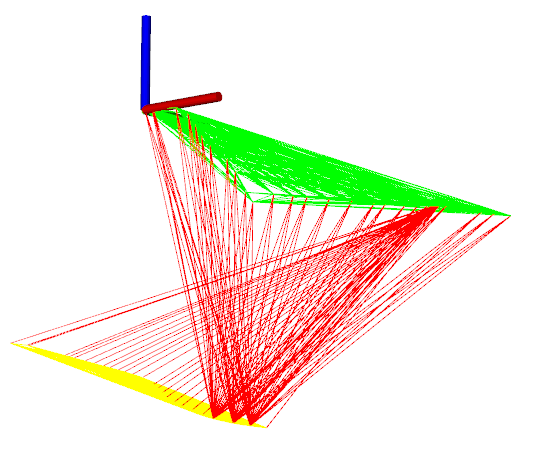
\includegraphics[scale=0.21]{gfx/covgraph_minHits_5_skip_1}}
    \subcaptionbox{10 \gls{kf} skipped after a \gls{kfm} was found}{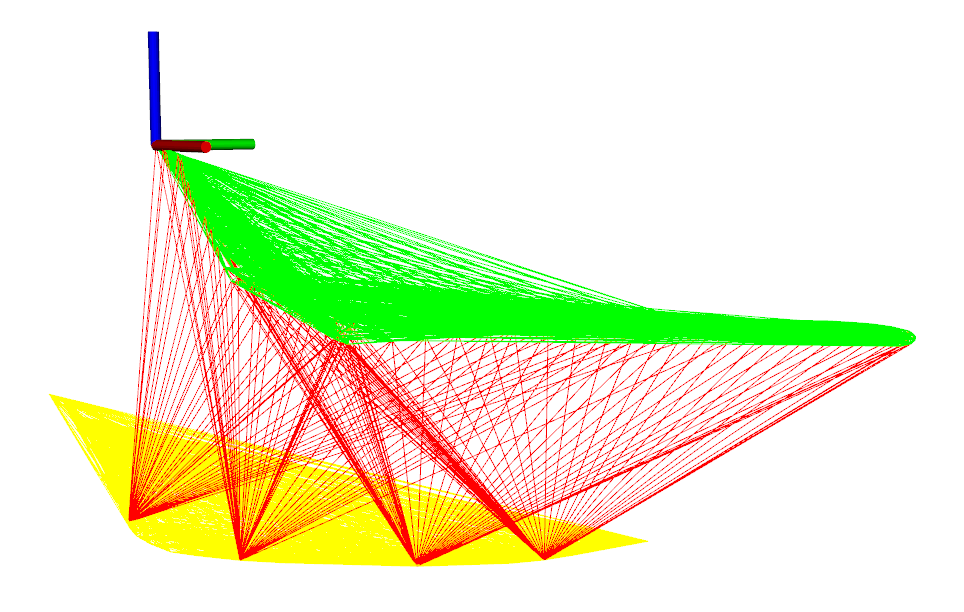
\includegraphics[scale=0.17]{gfx/covgraph_minHits_5_skip_10}}
  \end{figure}
  }
}

\frame{
  \frametitle{Map merging - Results - Reduction of drift}
  \begin{figure}[H]
    \centering
    \subcaptionbox{original approach}{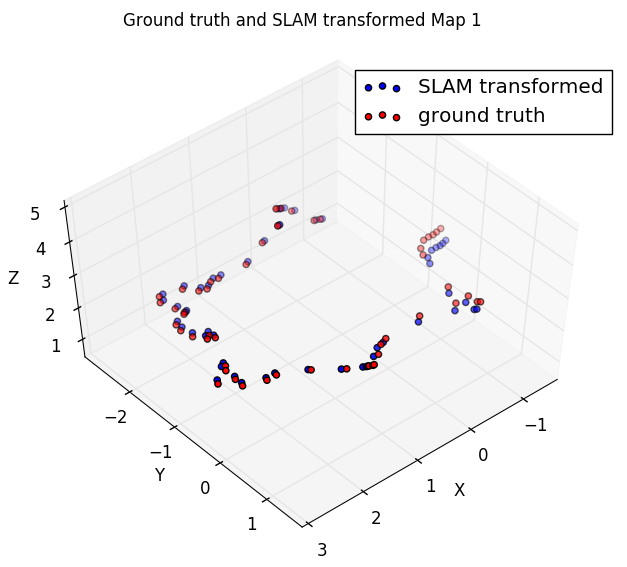
\includegraphics[scale=0.225]{gfx/m1_skf0_cut}}
    \subcaptionbox{new approach}{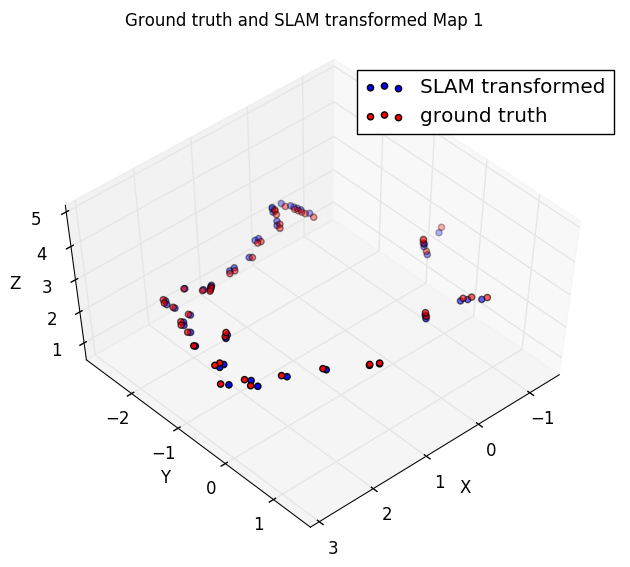
\includegraphics[scale=0.225]{gfx/m10_skf10_cut}}
  \end{figure}
  Reduction of the error from $\text{rmse} = 0.13\text{m}$ to $\text{rmse} = 0.10\text{m}$
}
\note[enumerate]
{
  \item Data set recorded with an \gls{uav} in VICON room
  \item Points represent \gls{kf} and the corresponding ground truth (VICON)
}

\section{Culling}
\frame{\tableofcontents[currentsection]}

\frame{
  \frametitle{Culling - Remove redundant \gls{kf}}
  \only<1>{
  \begin{block}{Motivation}
    Perform \acrfull{kf} culling to remove redundant information as bundle adjustment complexity grows with the number of \glspl{kf}
  \end{block}
  }
  \begin{itemize}
    \visible<2->{
    \item Remove redundant \glspl{kf} before map merging
    }
    \visible<3->{
    \item{Performs culling for every \gls{kfm} separately}
    }
  \end{itemize}

  \only<4>{
  \begin{center}
    \begin{tikzpicture}[auto]
    \coordinate (A1) at (-0.5, 0);
    \coordinate (KFM11) at (1, 0);
    \coordinate (A1MP1) at (-0.5, 0);
    \coordinate (A1MP2) at (0, 0);
    \coordinate (A1MP3) at (0.5, 0);
    \coordinate (A1MP4) at (1.5, 0);
    \coordinate (A1MP5) at (2, 0);
    \coordinate (A1MP6) at (2.5, 0);

    \coordinate (B1) at (6.5, 0);
    \coordinate (KFM12) at (5, 0);
    \coordinate (B1MP1) at (5.5, 0);
    \coordinate (B1MP2) at (6.0, 0);
    \coordinate (B1MP3) at (6.5, 0);
    \coordinate (B1MP4) at (4.5, 0);
    \coordinate (B1MP5) at (4.0, 0);
    \coordinate (B1MP6) at (3.5, 0);

    \coordinate (A2) at (-0.5, -3);
    \coordinate (KFM21) at (1, -3);
    \coordinate (A2MP1) at (-0.5, -3);
    \coordinate (A2MP2) at (0, -3);
    \coordinate (A2MP3) at (0.5, -3);
    \coordinate (A2MP4) at (1.5, -3);
    \coordinate (A2MP5) at (2, -3);
    \coordinate (A2MP6) at (2.5, -3);

    \coordinate (B2) at (6.5, -3);
    \coordinate (KFM22) at (5, -3);
    \coordinate (B2MP1) at (5.5, -3);
    \coordinate (B2MP2) at (6.0, -3);
    \coordinate (B2MP3) at (6.5, -3);
    \coordinate (B2MP4) at (4.5, -3);
    \coordinate (B2MP5) at (4.0, -3);
    \coordinate (B2MP6) at (3.5, -3);

    \node [fill=blue!30, circle,inner sep=2pt, text width=0.1mm] at (A1MP1) {};
    \node [fill=blue!30, circle,inner sep=2pt, text width=0.1mm] at (A1MP2) {};
    \node [fill=blue!30, circle,inner sep=2pt, text width=0.1mm] at (A1MP3) {};
    \node [fill=blue!70, circle,inner sep=3pt, text width=0.1mm] at (KFM11) {};
    \node [fill=blue!30, circle,inner sep=2pt, text width=0.1mm] at (A1MP4) {};
    \node [fill=blue!30, circle,inner sep=2pt, text width=0.1mm] at (A1MP5) {};
    \node [fill=blue!30, circle,inner sep=2pt, text width=0.1mm] at (A1MP6) {};

    \node [fill=blue!30, circle,inner sep=2pt, text width=0.1mm] at (B1MP1) {};
    \node [fill=blue!30, circle,inner sep=2pt, text width=0.1mm] at (B1MP2) {};
    \node [fill=blue!30, circle,inner sep=2pt, text width=0.1mm] at (B1MP3) {};
    \node [fill=blue!70, circle,inner sep=3pt, text width=0.1mm] at (KFM12) {};
    \node [fill=blue!30, circle,inner sep=2pt, text width=0.1mm] at (B1MP4) {};
    \node [fill=blue!30, circle,inner sep=2pt, text width=0.1mm] at (B1MP5) {};
    \node [fill=blue!30, circle,inner sep=2pt, text width=0.1mm] at (B1MP6) {};

    \node [fill=orange!30, circle,inner sep=2pt, text width=0.1mm] at (A2MP1) {};
    \node [fill=orange!30, circle,inner sep=2pt, text width=0.1mm] at (A2MP2) {};
    \node [fill=orange!30, circle,inner sep=2pt, text width=0.1mm] at (A2MP3) {};
    \node [fill=orange!70, circle,inner sep=3pt, text width=0.1mm] at (KFM21) {};
    \node [fill=orange!30, circle,inner sep=2pt, text width=0.1mm] at (A2MP4) {};
    \node [fill=orange!30, circle,inner sep=2pt, text width=0.1mm] at (A2MP5) {};
    \node [fill=orange!30, circle,inner sep=2pt, text width=0.1mm] at (A2MP6) {};

    \node [fill=orange!30, circle,inner sep=2pt, text width=0.1mm] at (B2MP1) {};
    \node [fill=orange!30, circle,inner sep=2pt, text width=0.1mm] at (B2MP2) {};
    \node [fill=orange!30, circle,inner sep=2pt, text width=0.1mm] at (B2MP3) {};
    \node [fill=orange!70, circle,inner sep=3pt, text width=0.1mm] at (KFM22) {};
    \node [fill=orange!30, circle,inner sep=2pt, text width=0.1mm] at (B2MP4) {};
    \node [fill=orange!30, circle,inner sep=2pt, text width=0.1mm] at (B2MP5) {};
    \node [fill=orange!30, circle,inner sep=2pt, text width=0.1mm] at (B2MP6) {};

    \draw [blue!50, line width=0.05cm] (A1) to (B1);
    \draw [orange!50, line width=0.05cm] (A2) to (B2);

    \draw [red!50, line width=0.05cm, dashed] (KFM11) to (KFM21);
    \draw [red!50, line width=0.05cm, dashed] (KFM12) to (KFM22);

    \node[draw] at (3.0, -4.25)
    {
    \scriptsize
    \begin{tabular}{cl}
      \tikz\node[fill=orange!70, circle,inner sep=3pt, text width=0.1mm] {}; \tikz\node[fill=blue!70, circle,inner sep=3pt, text width=0.1mm] {}; & KeyFrames of a Match \\
      \tikz\node[fill=orange!30, circle,inner sep=2.0pt, text width=0.1mm] {}; \tikz\node[fill=blue!30, circle,inner sep=2.0pt, text width=0.1mm] {}; & KeyFrames \\
    \end{tabular}
    };
    \end{tikzpicture}
%    \begin{tikzpicture}[auto]
%      \node[entity] (key frame match) {kf match}
%        [grow=down,sibling distance=4.5cm]
%        child {node[entity] (child 1) {kf, map 1}
%          [grow=down,sibling distance=1.2cm]
%          child {node[entity,minimum size=1cm] {kf 1}}
%          child {node[entity,minimum size=1cm] {kf 2}}
%          child {node[entity,minimum size=1cm] {kf $k$}}}
%        child {node[entity] {kf, map 2}
%          [grow=down,sibling distance=1.2cm]
%          child {node[entity,minimum size=1cm] {kf 1}}
%          child {node[entity,minimum size=1cm] {kf 2}}
%          child {node[entity,minimum size=1cm] {kf $l$}}};
%
%      \draw[blue,thick,dashed] (-2.25,-2.25) ellipse (1.5 and 0.5);
%      \draw[blue,thick,dashed] (2.25,-2.25) ellipse (1.5 and 0.5);
%      \draw[red,thick,dashed] (0,-2.25) ellipse (5 and 1.5);
%    \end{tikzpicture}
  \end{center}
  }

  \only<5>{
  \begin{center}
    \begin{tikzpicture}[auto]
    \coordinate (A1) at (-0.5, 0);
    \coordinate (KFM11) at (1, 0);
    \coordinate (A1MP1) at (-0.5, 0);
    \coordinate (A1MP2) at (0, 0);
    \coordinate (A1MP3) at (0.5, 0);
    \coordinate (A1MP4) at (1.5, 0);
    \coordinate (A1MP5) at (2, 0);
    \coordinate (A1MP6) at (2.5, 0);

    \coordinate (B1) at (6.5, 0);
    \coordinate (KFM12) at (5, 0);
    \coordinate (B1MP1) at (5.5, 0);
    \coordinate (B1MP2) at (6.0, 0);
    \coordinate (B1MP3) at (6.5, 0);
    \coordinate (B1MP4) at (4.5, 0);
    \coordinate (B1MP5) at (4.0, 0);
    \coordinate (B1MP6) at (3.5, 0);

    \coordinate (A2) at (-0.5, -3);
    \coordinate (KFM21) at (1, -3);
    \coordinate (A2MP1) at (-0.5, -3);
    \coordinate (A2MP2) at (0, -3);
    \coordinate (A2MP3) at (0.5, -3);
    \coordinate (A2MP4) at (1.5, -3);
    \coordinate (A2MP5) at (2, -3);
    \coordinate (A2MP6) at (2.5, -3);

    \coordinate (B2) at (6.5, -3);
    \coordinate (KFM22) at (5, -3);
    \coordinate (B2MP1) at (5.5, -3);
    \coordinate (B2MP2) at (6.0, -3);
    \coordinate (B2MP3) at (6.5, -3);
    \coordinate (B2MP4) at (4.5, -3);
    \coordinate (B2MP5) at (4.0, -3);
    \coordinate (B2MP6) at (3.5, -3);

    \node [fill=blue!30, circle,inner sep=2pt, text width=0.1mm] at (A1MP1) {};
    \node [fill=blue!30, circle,inner sep=2pt, text width=0.1mm] at (A1MP2) {};
    \node [fill=blue!30, circle,inner sep=2pt, text width=0.1mm] at (A1MP3) {};
    \node [fill=blue!70, circle,inner sep=3pt, text width=0.1mm] at (KFM11) {};
    \node [fill=blue!30, circle,inner sep=2pt, text width=0.1mm] at (A1MP4) {};
    \node [fill=blue!30, circle,inner sep=2pt, text width=0.1mm] at (A1MP5) {};
    \node [fill=blue!30, circle,inner sep=2pt, text width=0.1mm] at (A1MP6) {};

    \node [fill=blue!30, circle,inner sep=2pt, text width=0.1mm] at (B1MP1) {};
    \node [fill=blue!30, circle,inner sep=2pt, text width=0.1mm] at (B1MP2) {};
    \node [fill=blue!30, circle,inner sep=2pt, text width=0.1mm] at (B1MP3) {};
    \node [fill=blue!70, circle,inner sep=3pt, text width=0.1mm] at (KFM12) {};
    \node [fill=blue!30, circle,inner sep=2pt, text width=0.1mm] at (B1MP4) {};
    \node [fill=blue!30, circle,inner sep=2pt, text width=0.1mm] at (B1MP5) {};
    \node [fill=blue!30, circle,inner sep=2pt, text width=0.1mm] at (B1MP6) {};

    \node [fill=orange!30, circle,inner sep=2pt, text width=0.1mm] at (A2MP1) {};
    \node [fill=orange!30, circle,inner sep=2pt, text width=0.1mm] at (A2MP2) {};
    \node [fill=orange!30, circle,inner sep=2pt, text width=0.1mm] at (A2MP3) {};
    \node [fill=orange!70, circle,inner sep=3pt, text width=0.1mm] at (KFM21) {};
    \node [fill=orange!30, circle,inner sep=2pt, text width=0.1mm] at (A2MP4) {};
    \node [fill=orange!30, circle,inner sep=2pt, text width=0.1mm] at (A2MP5) {};
    \node [fill=orange!30, circle,inner sep=2pt, text width=0.1mm] at (A2MP6) {};

    \node [fill=orange!30, circle,inner sep=2pt, text width=0.1mm] at (B2MP1) {};
    \node [fill=orange!30, circle,inner sep=2pt, text width=0.1mm] at (B2MP2) {};
    \node [fill=orange!30, circle,inner sep=2pt, text width=0.1mm] at (B2MP3) {};
    \node [fill=orange!70, circle,inner sep=3pt, text width=0.1mm] at (KFM22) {};
    \node [fill=orange!30, circle,inner sep=2pt, text width=0.1mm] at (B2MP4) {};
    \node [fill=orange!30, circle,inner sep=2pt, text width=0.1mm] at (B2MP5) {};
    \node [fill=orange!30, circle,inner sep=2pt, text width=0.1mm] at (B2MP6) {};

    \draw [blue!50, line width=0.05cm] (A1) to (B1);
    \draw [orange!50, line width=0.05cm] (A2) to (B2);

    \draw [red!50, line width=0.05cm, dashed] (KFM11) to (KFM21);
    \draw [red!50, line width=0.05cm, dashed] (KFM12) to (KFM22);

    \draw[black,thick,dashed] (-1, 0.5) -- (2.9, 0.5) -- (2.9, -3.5) -- (-1, -3.5) -- (-1, 0.5);
    \draw[black,thick,dashed] (3.1, 0.5) -- (7.0, 0.5) -- (7.0, -3.5) -- (3.1, -3.5) -- (3.1, 0.5);

    \node[draw] at (3.0, -4.25)
    {
    \scriptsize
    \begin{tabular}{cl}
      \tikz\node[fill=orange!70, circle,inner sep=3pt, text width=0.1mm] {}; \tikz\node[fill=blue!70, circle,inner sep=3pt, text width=0.1mm] {}; & KeyFrames of a Match \\
      \tikz\node[fill=orange!30, circle,inner sep=2.0pt, text width=0.1mm] {}; \tikz\node[fill=blue!30, circle,inner sep=2.0pt, text width=0.1mm] {}; & KeyFrames \\
    \end{tabular}
    };
    \end{tikzpicture}
  \end{center}
  }

  \only<6>{
  \begin{center}
    \begin{tikzpicture}[auto]
    \coordinate (A1) at (-0.5, 0);
    \coordinate (KFM11) at (1, 0);
    \coordinate (A1MP1) at (-0.5, 0);
    \coordinate (A1MP2) at (0, 0);
    \coordinate (A1MP3) at (0.5, 0);
    \coordinate (A1MP4) at (1.5, 0);
    \coordinate (A1MP5) at (2, 0);
    \coordinate (A1MP6) at (2.5, 0);

    \coordinate (B1) at (6.5, 0);
    \coordinate (KFM12) at (5, 0);
    \coordinate (B1MP1) at (5.5, 0);
    \coordinate (B1MP2) at (6.0, 0);
    \coordinate (B1MP3) at (6.5, 0);
    \coordinate (B1MP4) at (4.5, 0);
    \coordinate (B1MP5) at (4.0, 0);
    \coordinate (B1MP6) at (3.5, 0);

    \coordinate (A2) at (-0.5, -3);
    \coordinate (KFM21) at (1, -3);
    \coordinate (A2MP1) at (-0.5, -3);
    \coordinate (A2MP2) at (0, -3);
    \coordinate (A2MP3) at (0.5, -3);
    \coordinate (A2MP4) at (1.5, -3);
    \coordinate (A2MP5) at (2, -3);
    \coordinate (A2MP6) at (2.5, -3);

    \coordinate (B2) at (6.5, -3);
    \coordinate (KFM22) at (5, -3);
    \coordinate (B2MP1) at (5.5, -3);
    \coordinate (B2MP2) at (6.0, -3);
    \coordinate (B2MP3) at (6.5, -3);
    \coordinate (B2MP4) at (4.5, -3);
    \coordinate (B2MP5) at (4.0, -3);
    \coordinate (B2MP6) at (3.5, -3);

    \node [red] at (A1MP1) {$\boldsymbol{\times}$};
    \node [fill=blue!30, circle,inner sep=2pt, text width=0.1mm] at (A1MP2) {};
    \node [fill=blue!30, circle,inner sep=2pt, text width=0.1mm] at (A1MP3) {};
    \node [fill=blue!70, circle,inner sep=3pt, text width=0.1mm] at (KFM11) {};
    \node [red] at (A1MP4) {$\boldsymbol{\times}$};
    \node [fill=blue!30, circle,inner sep=2pt, text width=0.1mm] at (A1MP5) {};
    \node [fill=blue!30, circle,inner sep=2pt, text width=0.1mm] at (A1MP6) {};

    \node [fill=blue!30, circle,inner sep=2pt, text width=0.1mm] at (B1MP1) {};
    \node [red] at (B1MP2) {$\boldsymbol{\times}$};
    \node [fill=blue!30, circle,inner sep=2pt, text width=0.1mm] at (B1MP3) {};
    \node [fill=blue!70, circle,inner sep=3pt, text width=0.1mm] at (KFM12) {};
    \node [fill=blue!30, circle,inner sep=2pt, text width=0.1mm] at (B1MP4) {};
    \node [fill=blue!30, circle,inner sep=2pt, text width=0.1mm] at (B1MP5) {};
    \node [fill=blue!30, circle,inner sep=2pt, text width=0.1mm] at (B1MP6) {};

    \node [fill=orange!30, circle,inner sep=2pt, text width=0.1mm] at (A2MP1) {};
    \node [fill=orange!30, circle,inner sep=2pt, text width=0.1mm] at (A2MP2) {};
    \node [red] at (A2MP3) {$\boldsymbol{\times}$};
    \node [fill=orange!70, circle,inner sep=3pt, text width=0.1mm] at (KFM21) {};
    \node [fill=orange!30, circle,inner sep=2pt, text width=0.1mm] at (A2MP4) {};
    \node [fill=orange!30, circle,inner sep=2pt, text width=0.1mm] at (A2MP5) {};
    \node [fill=orange!30, circle,inner sep=2pt, text width=0.1mm] at (A2MP6) {};

    \node [fill=orange!30, circle,inner sep=2pt, text width=0.1mm] at (B2MP1) {};
    \node [fill=orange!30, circle,inner sep=2pt, text width=0.1mm] at (B2MP2) {};
    \node [fill=orange!30, circle,inner sep=2pt, text width=0.1mm] at (B2MP3) {};
    \node [fill=orange!70, circle,inner sep=3pt, text width=0.1mm] at (KFM22) {};
    \node [fill=orange!30, circle,inner sep=2pt, text width=0.1mm] at (B2MP4) {};
    \node [fill=orange!30, circle,inner sep=2pt, text width=0.1mm] at (B2MP5) {};
    \node [red] at (B2MP6) {$\boldsymbol{\times}$};

    \draw [blue!50, line width=0.05cm] (A1) to (B1);
    \draw [orange!50, line width=0.05cm] (A2) to (B2);

    \draw [red!50, line width=0.05cm, dashed] (KFM11) to (KFM21);
    \draw [red!50, line width=0.05cm, dashed] (KFM12) to (KFM22);

    \draw[black,thick,dashed] (-1, 0.5) -- (2.9, 0.5) -- (2.9, -3.5) -- (-1, -3.5) -- (-1, 0.5);
    \draw[black,thick,dashed] (3.1, 0.5) -- (7.0, 0.5) -- (7.0, -3.5) -- (3.1, -3.5) -- (3.1, 0.5);

    \node[draw] at (3.0, -4.25)
    {
    \scriptsize
    \begin{tabular}{cl}
      \tikz\node[fill=orange!70, circle,inner sep=3pt, text width=0.1mm] {}; \tikz\node[fill=blue!70, circle,inner sep=3pt, text width=0.1mm] {}; & KeyFrames of a Match \\
      \tikz\node[fill=orange!30, circle,inner sep=2.0pt, text width=0.1mm] {}; \tikz\node[fill=blue!30, circle,inner sep=2.0pt, text width=0.1mm] {}; & KeyFrames \\
    \end{tabular}
    };
    \end{tikzpicture}
  \end{center}
  }
}
\note{ORB-SLAM Culling approach}

\subsection{Results}

\frame{
  \frametitle{Culling - Results}
  \visible<1->{
  Culling removes $\approx 13$\% of the \acrfullpl{kf}\\
  }

  \visible<2->{
  \smallskip

  \begin{table}[ht!]
  \begin{center}
  \begin{tabular}{c|c|c|c|c}
    Culling &  \# \glspl{kfm} & \# \glspl{kf} skipped & \acrshort{pgo} [ms] & \acrshort{ba} [ms] \\ 
    \hline
    No & 10 & 10 & \textcolor{cyan}{532.28} & \textcolor{magenta}{3659.48} \\
    Yes & 10 & 10 & \textcolor{cyan}{178.83} & \textcolor{magenta}{1098.37} \\
    %\hline 
  \end{tabular}
  \end{center}
  \caption{Time measurements of \gls{pgo} and \gls{ba} without and with culling.}
  \label{tab:results_time}
  \end{table}
  }

  \visible<3>{
    \begin{block}{}
      Performance increases significantly when culling is enabled
    \end{block}
  }
  {\small\acrfull{pgo}}\\
  {\small\acrfull{ba}}\\
}

\frame{
  \frametitle{Culling - Results}
  \visible<1-2>{
  \begin{table}[ht!]
  \begin{center}
  \begin{tabular}{c|c|c|c}
    Culling &  \# \glspl{kfm} & \# \glspl{kf} skipped & \textit{rmse} [m] \\ 
    \hline \hline
    No & 1 & 0 & 0.1311 \\
    Yes & 1 & 0 & \textcolor{red}{0.2187} \\
    \hline
    No & 10 & 10 & 0.0961 \\
    Yes & 10 & 10 & \textcolor{blue}{0.0965} \\
    %\hline 
  \end{tabular}
  \end{center}
  \caption{\textit{rmse} without and with culling.}
  \label{tab:results_rmse}
  \end{table}
  }

  \visible<2>{
    \begin{block}{}
      Accuracy gets worse if not enough information is available.\\No problem with multiple \acrfullpl{kfm}.
    \end{block}
  }
}

\section{Optimization}
\frame{\tableofcontents[currentsection]}

\frame{
  \frametitle{Optimization - Idea}
  \visible<1->{
  \begin{block}{}
  Considerable computational benefits can be gained by substituting the \acrfull{lm} algorithm in the implementation of \acrfull{ba} with a variant of \acrfull{dl} non-linear least squares technique \cite{Lourakis2005}
  \end{block}
  }
  \only<2>{
  \acrshort{dl} optimizer handles trust region differently
  }
}

\frame{
  \frametitle{Optimization - Approach}
  \begin{itemize}
    \visible<1-4>{
    \item Tried \acrfull{pgo} and \acrfull{ba} with the \acrfull{dl} optimizer.
    }
    \visible<2-4>{
    \item \gls{pgo}: Slightly worse timing using the \gls{dl} optimizer
    }
    \visible<3-4>{
    \item \gls{ba}: Better timing using the \gls{dl} optimizer
    }
  \end{itemize}

  \visible<4>{
  \begin{block}{Conclusion}
    \gls{lm} optimizer for \gls{pgo} and \gls{dl} optimizer for \gls{ba}
  \end{block}
  }
}

\subsection{Results}

\frame{
  \frametitle{Optimization - Results}
  \visible<1-2>{

  \begin{table}[ht!]
  \begin{center}
  \begin{tabular}{c|c|c|c|c}
    Opt. & \# \glspl{kfm} & \# \glspl{kf} skipped & \gls{pgo} [ms] & \gls{ba} [ms] \\ 
    \hline
    \gls{lm}/\gls{lm} & 10 & 10 & \textcolor{cyan}{178.83} & \textcolor{magenta}{1098.37} \\
    \gls{lm}/\gls{dl} & 10 & 10 & \textcolor{cyan}{178.70} & \textcolor{magenta}{383.54} \\
    %\hline 
  \end{tabular}
  \end{center}
  \caption{Time measurements of \gls{lm} and \gls{dl} optimizer.}
  \label{tab:results_dogleg_time}
  \end{table}
  }

  \visible<2>{
  \begin{block}{}
    Accuracy stays the same while the performance is increased
  \end{block}
  }
  {\small\acrfull{pgo}}\\
  {\small\acrfull{ba}}\\
}

\section{Conclusion}
\frame{\tableofcontents[currentsection]}

\begin{frame}
	\frametitle{Conclusion}
	\only<1-2>{
	\begin{itemize}
		  \visible<1-2>{\item Multiple \glspl{kfm} approach increases accuracy}
		  \visible<2>{\item Skipping of \glspl{kf} spreads \glspl{kfm} over a bigger area}
	\end{itemize}
	}
	\only<3-6>{
    \begin{block}{Higher accuracy}
	 The use of \glspl{kfm} from a bigger area serves \gls{pgo} and \gls{ba} with more information $\rightarrow$ higher accuracy
    \end{block}
	}

	\only<4-5>{
	\begin{itemize}
		\visible<4-5>{\item Culling removes redundant \glspl{kf} $\rightarrow$ improved timing}
		\visible<5>{\item Using \gls{dl} optimizer for the \gls{ba} also improves timing}
	\end{itemize}
	}

  \only<6>{
    \begin{block}{Better timing}
      Culling and the use of the \gls{dl} optimizer improves timing
    \end{block}
  }
\end{frame}

\section{Outlook}

\frame{\tableofcontents[currentsection]}

\frame { \frametitle{Outlook \& Limitation}
  \visible<1->{
	\pause
  Outlook:\\
	\begin{itemize}
	\pause
  \item Heuristic for best map alignment
	\pause
  \item Extend area for \gls{kf} culling
	\end{itemize}
  }
  \visible<1->{
	\pause
  Limitation:\\
	\begin{itemize}
	\pause
  \item \# of \glspl{kfm} and \# of skips depends on data set
	\end{itemize}
  }
}
\note[itemize]
{
  \item Heuristic: Based on reprojection error
  \item Extend area: Second order neighbors
}

%\section{Q\&A}
\frame { \frametitle{Q\&A}
	\begin{center}
	
\includegraphics[height=0.75\textheight]{gfx/q&a.jpg}
	\end{center}
}

%\section{References}
\frame{ \frametitle{References}
	\bibliography{references}
}

\end{document}
